\documentclass[paper=a4wide, fontsize=11pt]{report}	 % A4 paper and 11pt font size
\usepackage[svgnames]{xcolor} % Using colors
\usepackage{xurl} %xurl en vez de url para urls largas
\usepackage[hidelinks]{hyperref}
\usepackage[utf8]{inputenc}
\renewcommand\thechapter{\Roman{chapter}}
\usepackage[spanish]{babel} % ponerlo en español
\usepackage{todonotes} % para poner notitas de colores
\usepackage{fancyhdr} % Needed to define custom headers/footers
\usepackage[a4paper, left=30mm, right=30mm, top=2.5cm, bottom=2.5cm, footskip=1.2cm]{geometry}  % Changing size of document
\usepackage{braket}
\usepackage{tabularx}
\usepackage{multirow}
\usepackage{nicematrix}
\usepackage[numbers]{natbib}
\usepackage{subcaption}
\usepackage{tabularx, makecell, booktabs}
\usepackage{textcmds}
\usepackage{color}
\usepackage{listings}
\definecolor{lightgray}{rgb}{.9,.9,.9}
\definecolor{darkgray}{rgb}{.4,.4,.4}
\definecolor{purple}{rgb}{0.65, 0.12, 0.82}
%%%%%% Setting up the style

\pagestyle{fancy} % Enables the custom headers/footers

\lhead{} \rhead{} % Headers - all  empty



\title{
{\Huge \textbf{Proyecto: 
\\ Sistemas de Información 2}}\\
\vspace{1cm}
\vspace{1cm}
\text{Pablo Angusto\quad\href{mailto:842255@unizar.es}{842255@unizar.es}}\\
\text{Miguel Aréjula\quad\href{mailto:850068@unizar.es}{850068@unizar.es}}\\

\includegraphics[width=6cm]{logo.png}\\
\date{6 de marzo de 2024}



}


\cfoot{\color{Black} \thepage}

\renewcommand{\headrulewidth}{0.0pt} % No header rule
\renewcommand{\footrulewidth}{0.4pt} % Thin footer rule
\renewcommand{\thesection}{\arabic{section}} % para que los títulos no salgan en 0.1 ...

\setcounter{secnumdepth}{3}
%%%%%% Starting the document
\setlength\parindent{0pt} % No indentar los párrafos
\begin{document}
\author{Pablo Angusto and Miguel Aréjula}
\maketitle % Print the title
\tableofcontents
\newpage
\thispagestyle{fancy} % Enabling the custom headers/footers for the first page

% In the following lines, add the relevant information
\vspace{-0.5cm}

%TODO add content
\section{Introducción}

Odoo es un software de código abierto para la gestión empresarial. Destaca por ser una plataforma versátil con diversas áreas funcionales de una organización. Con un enfoque modular, Odoo ofrece una gran cantidad de aplicaciones; contabilidad, recursos humanos, ventas, inventario, CRM y más, permitiendo a las empresas optimizar sus procesos y centralizar su gestión.


Esta software modular facilita a las empresas la adaptación a sus necesidades específicas. La interfaz intuitiva y la naturaleza de código abierto de Odoo fomentan la personalización y la innovación continua, brindando a las empresas la flexibilidad necesaria para evolucionar con el cambiante panorama empresarial. Odoo está posicionada como una herramienta valiosa para impulsar el crecimiento y la eficacia operativa de las organizaciones.

\section{Instalación}
\paragraph{}
UZ-On-Marketing esta buscando introducir un ERP en su empresa. Algunas de las posiblidades son SAP, SAGE u Odoo. La empresa no dispone de mucho presupuesto para invertir en el ERP, por lo tanto, se ha decido utilizar la versión 17 de Odoo al ser de código abierto y tener coste cero.

\paragraph{}
Para instalar Odoo en las máquinas de la empresa hay varias opciones: instalar en paquetes, instalación en linea, instalación de origen o mediante Docker.
Hemos decidido instalarlo mediante docker ya que es una manera sencilla y rápida de obtener Odoo. 
Para ello es necesario tener instalado docker en nuestra máquina. En caso que no lo tengamos, podemos obtenerlo de diversas formas en función del  sistema operativo que tenga la máquina: 
\subsection{Instalación Docker}
\begin{itemize}
    \item \textbf{Windows:} 
    \begin{enumerate}
        \item Descarga Docker Desktop desde el sitio oficial de Docker: Docker Desktop for Windows.
        \item Ejecuta el instalador descargado y sigue las instrucciones del asistente de instalación.
        \item Durante la instalación, se te pedirá que habilites la virtualización en la BIOS de tu computadora, si aún no está habilitada. Asegúrate de seguir estas instrucciones si es necesario.
        \item Una vez completada la instalación, reinicia tu ordenador si es necesario.
    \end{enumerate}
    \item \textbf{MacOS: }
    \begin{enumerate}
        \item Descarga Docker Desktop desde el sitio oficial de Docker: Docker Desktop for Mac.
        \item Ejecuta el instalador descargado y arrastra el ícono de Docker a la carpeta de Aplicaciones.
        \item Abre Docker Desktop desde la carpeta de Aplicaciones.
    \end{enumerate}
    \item \textbf{Linux:} 
    \begin{itemize}
        \item \textbf{Sistemas basados en Debian (ej:Ubuntu)}
        \begin{enumerate}
            \item Actualiza el índice de paquetes: 
            \begin{lstlisting}[frame=single, basicstyle=\small]
sudo apt update
            \end{lstlisting}
            \item Instala paquetes para permitir que APT use un repositorio sobre HTTPS:
            \begin{lstlisting}[frame=single, basicstyle=\small]
sudo apt install apt-transport-https ca-certificates curl
software-properties-common
            \end{lstlisting}
            
            \item Agrega la clave GPG para el repositorio oficial de Docker:
            \begin{lstlisting}[frame=single, basicstyle=\small]
curl -fsSL https://download.docker.com/linux/ubuntu/gpg | sudo 
gpg --dearmor -o /usr/share/keyrings/docker-archive-keyring.gpg
            \end{lstlisting}
            
            \item Agrega el repositorio de Docker al sistema:
            \begin{lstlisting}[frame=single, basicstyle=\tiny]
echo "deb [signed-by=/usr/share/keyrings/docker-archive-keyring.gpg]
https://download.docker.com/linux/ubuntu \$(lsb\_release -cs) stable"
| sudo tee /etc/apt/sources.list.d/docker.list > /dev/null
            \end{lstlisting}
            
            \item Actualiza el índice de paquetes nuevamente:
           \begin{lstlisting}[frame=single, basicstyle=\small]
sudo apt update
            \end{lstlisting}
            \item Instala Docker:
            \begin{lstlisting}[frame=single, basicstyle=\small]
sudo apt install docker-ce docker-ce-cli containerd.io
            \end{lstlisting}
        \end{enumerate}
        \item \textbf{Sistemas basados en Red Hat (ej:Fedora)}
        \begin{enumerate}
            \item Instala Docker utilizando el gestor de paquetes dnf:
            \begin{lstlisting}[frame=single, basicstyle=\small]
sudo dnf install docker
            \end{lstlisting}
            \item Inicia y habilita el servicio Docker:
            \begin{lstlisting}[frame=single, basicstyle=\small]
sudo systemctl start docker
sudo systemctl enable docker
            \end{lstlisting}
        \end{enumerate}
        Para verificar que se ha instalado correctamente Docker ejecuta el comando:
        \begin{lstlisting}[frame=single, basicstyle=\small]
docker --version
        \end{lstlisting}
             Finalmente, para poder utilizar docker se va a necesitar los permisos de administrador por lo que puedes usar sudo o añadir tu usuario al grupo "docker" mediante el comando:
              \begin{lstlisting}[frame=single, basicstyle=\small]
sudo usermod -aG docker user.
        \end{lstlisting}
    \end{itemize}
\end{itemize}
\subsection{Instalación Odoo}
\paragraph{}
Una vez instalado docker, se va a continuar con la instalación de Odoo. El siguiente paso es crear un fichero con el nombre docker-compose.yml
\begin{lstlisting}[frame=single, basicstyle=\small]
version: "3.1"
services:
  odoo:
    image: odoo:17.0
    depends_on:
      - db
    ports:
      - "8069:8069"
    volumes:
      - odoo-web-data:/var/lib/odoo
    environment:
      - HOST=db
      - USER=odoo
      - PASSWORD=myodoo
  db:
    image: postgres:13
    environment:
      - POSTGRES_DB=postgres
      - POSTGRES_PASSWORD=myodoo
      - POSTGRES_USER=odoo
      - PGDATA=/var/lib/postgresql/data/pgdata
    volumes:
      - odoo-db-data:/var/lib/postgresql/data/pgdata
volumes:
  odoo-web-data:
  odoo-db-data:
\end{lstlisting}
\paragraph{}
A continuación, se necesita abrir una terminal y dirigerte al directorio donde se localiza el fichero docker-compose.yml. Para arrancar Odoo ejecuta en la terminal el comando docker compose up –d. Además, si se quiere parar Odoo se deberá ejecutar el comando docker compose stop o eliminarlo con docker compose down. Tras arrancar Odoo, para acceder a él se debe ir al navegador instalado en la máquina y escribir en la barra de busqueda de la parte superior la dirección http://localhost:8069/.
Redirige a /web/database/selector??? e introducir la siguiente información en el formulario, pulsar en create database y esperar a que se cree la base de datos.
\begin{figure}[h]
    \centering
    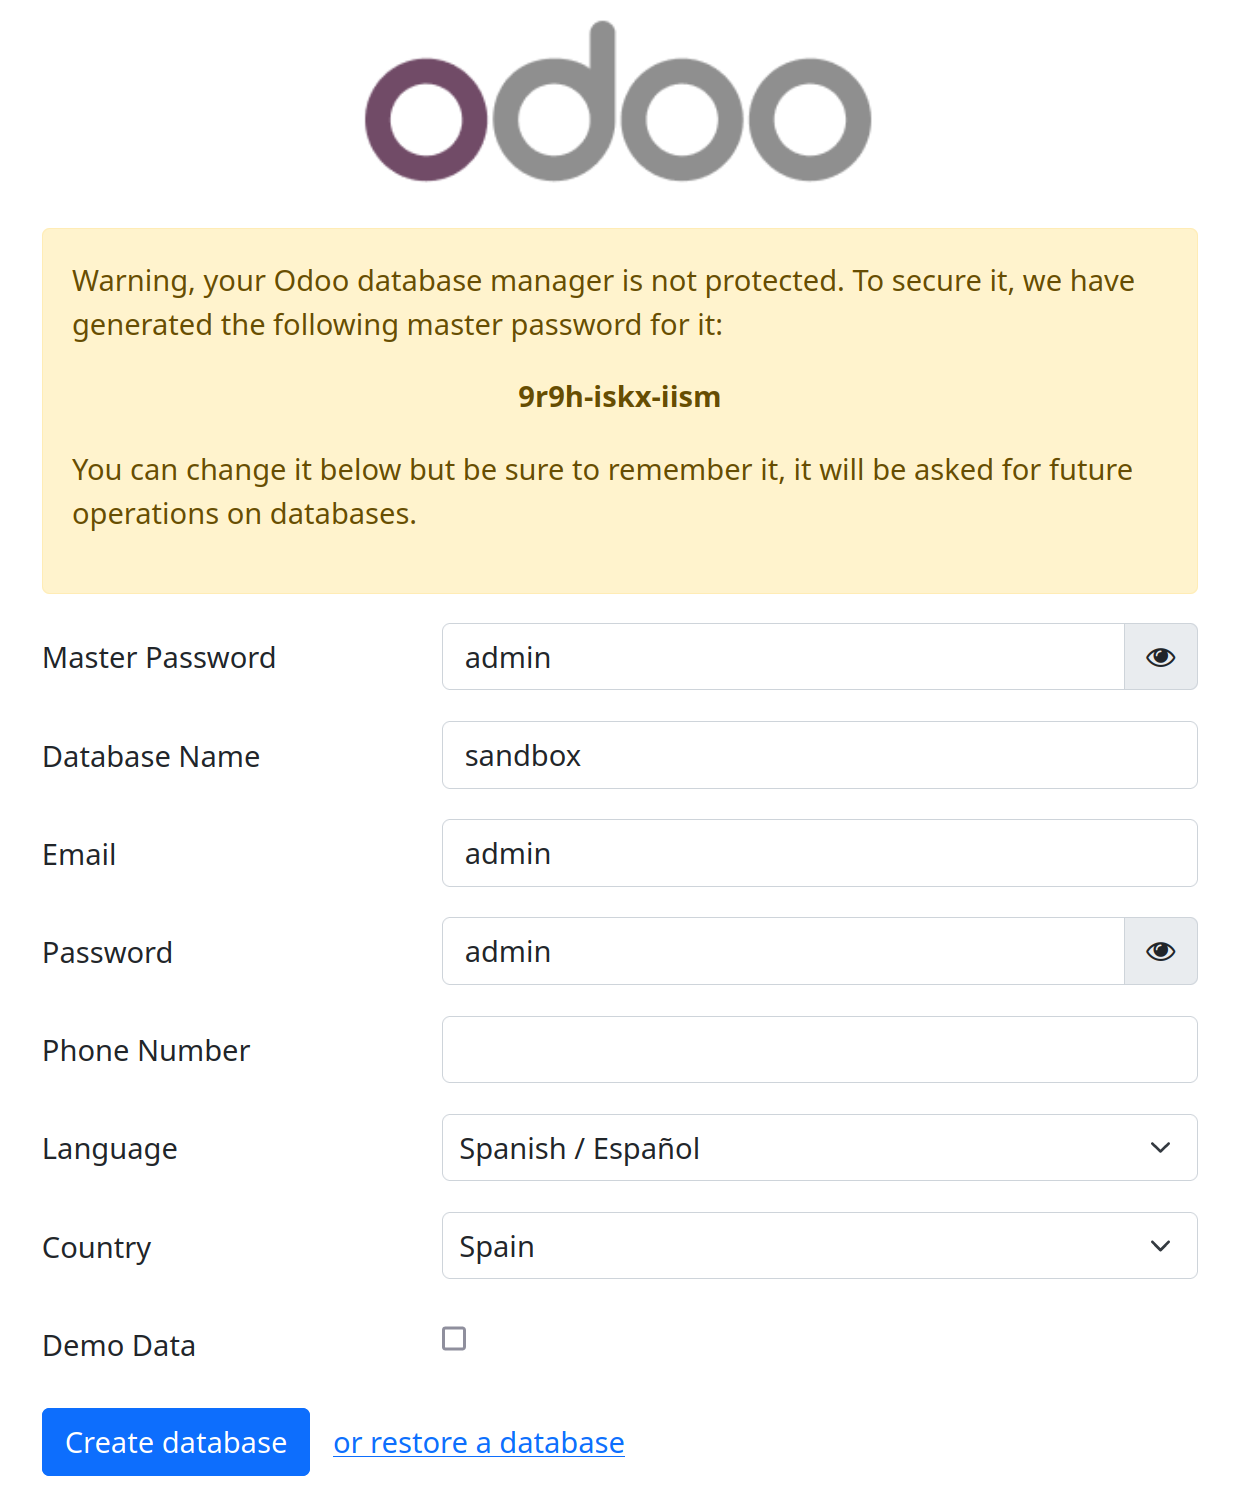
\includegraphics[width=6cm]{signup.png}
    \caption{Proceso de registro en Odoo}
    \label{fig:signup}
\end{figure}
Por último, cuando se tenga que iniciar sesión se tendrá que introducir el usuario admin y la contraseña admin.
\paragraph{}
Una vez dentro de Odoo, elimina el filtro de Aplicaciones de la barra de búsqueda y busca Blog.
\begin{figure}[h]
    \centering
    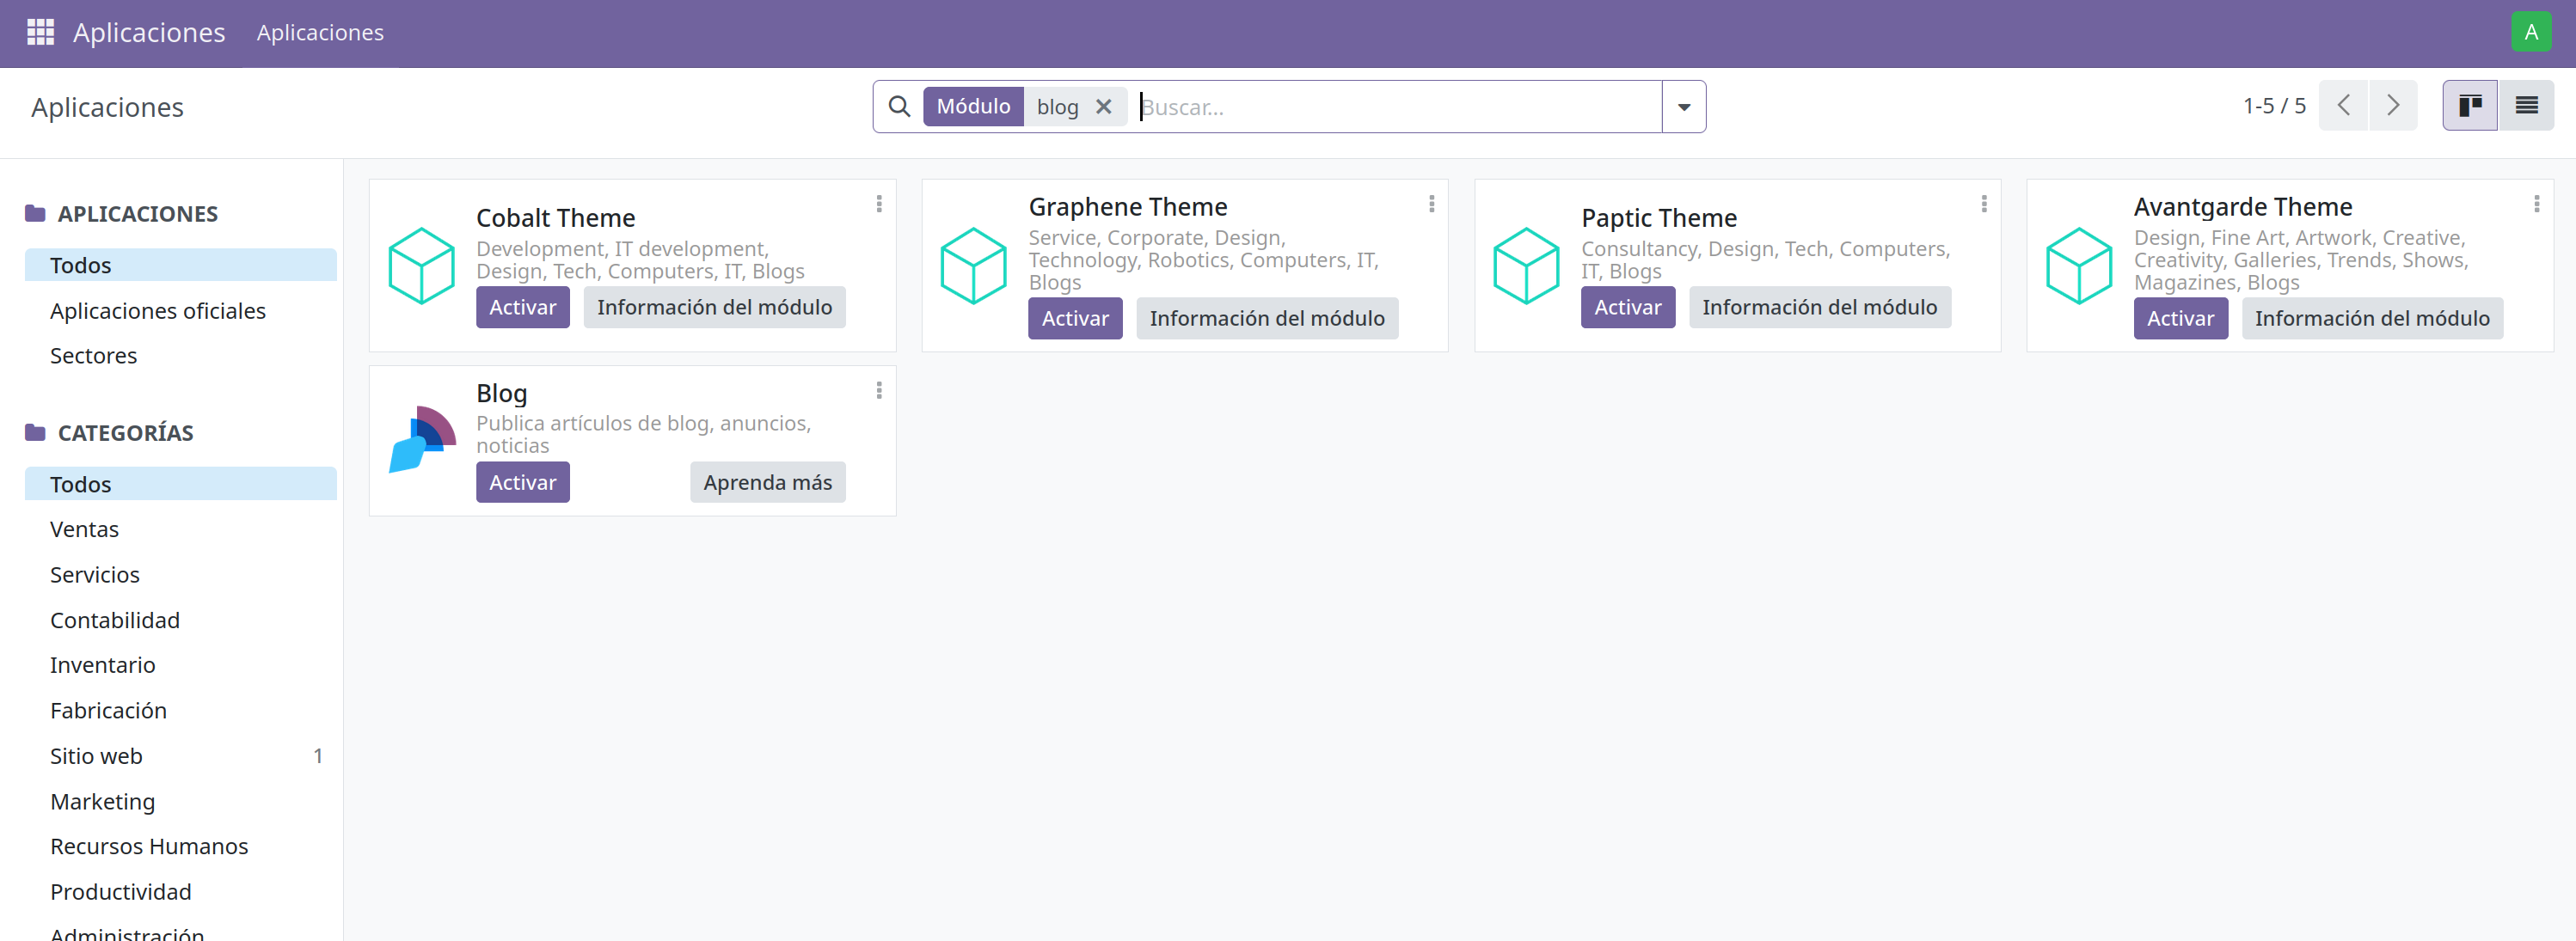
\includegraphics[width=6cm]{blog.png}
    \caption{Busqueda y activación del Blog}
    \label{fig:blog}
\end{figure}
\paragraph{}
Haz click en Activar dentro de la tarjeta de Blog, de esta manera se instalará automáticamente los módulos relacionados con la web. Se mostrará la siguiente pantalla:
\begin{figure}[h]
    \centering
    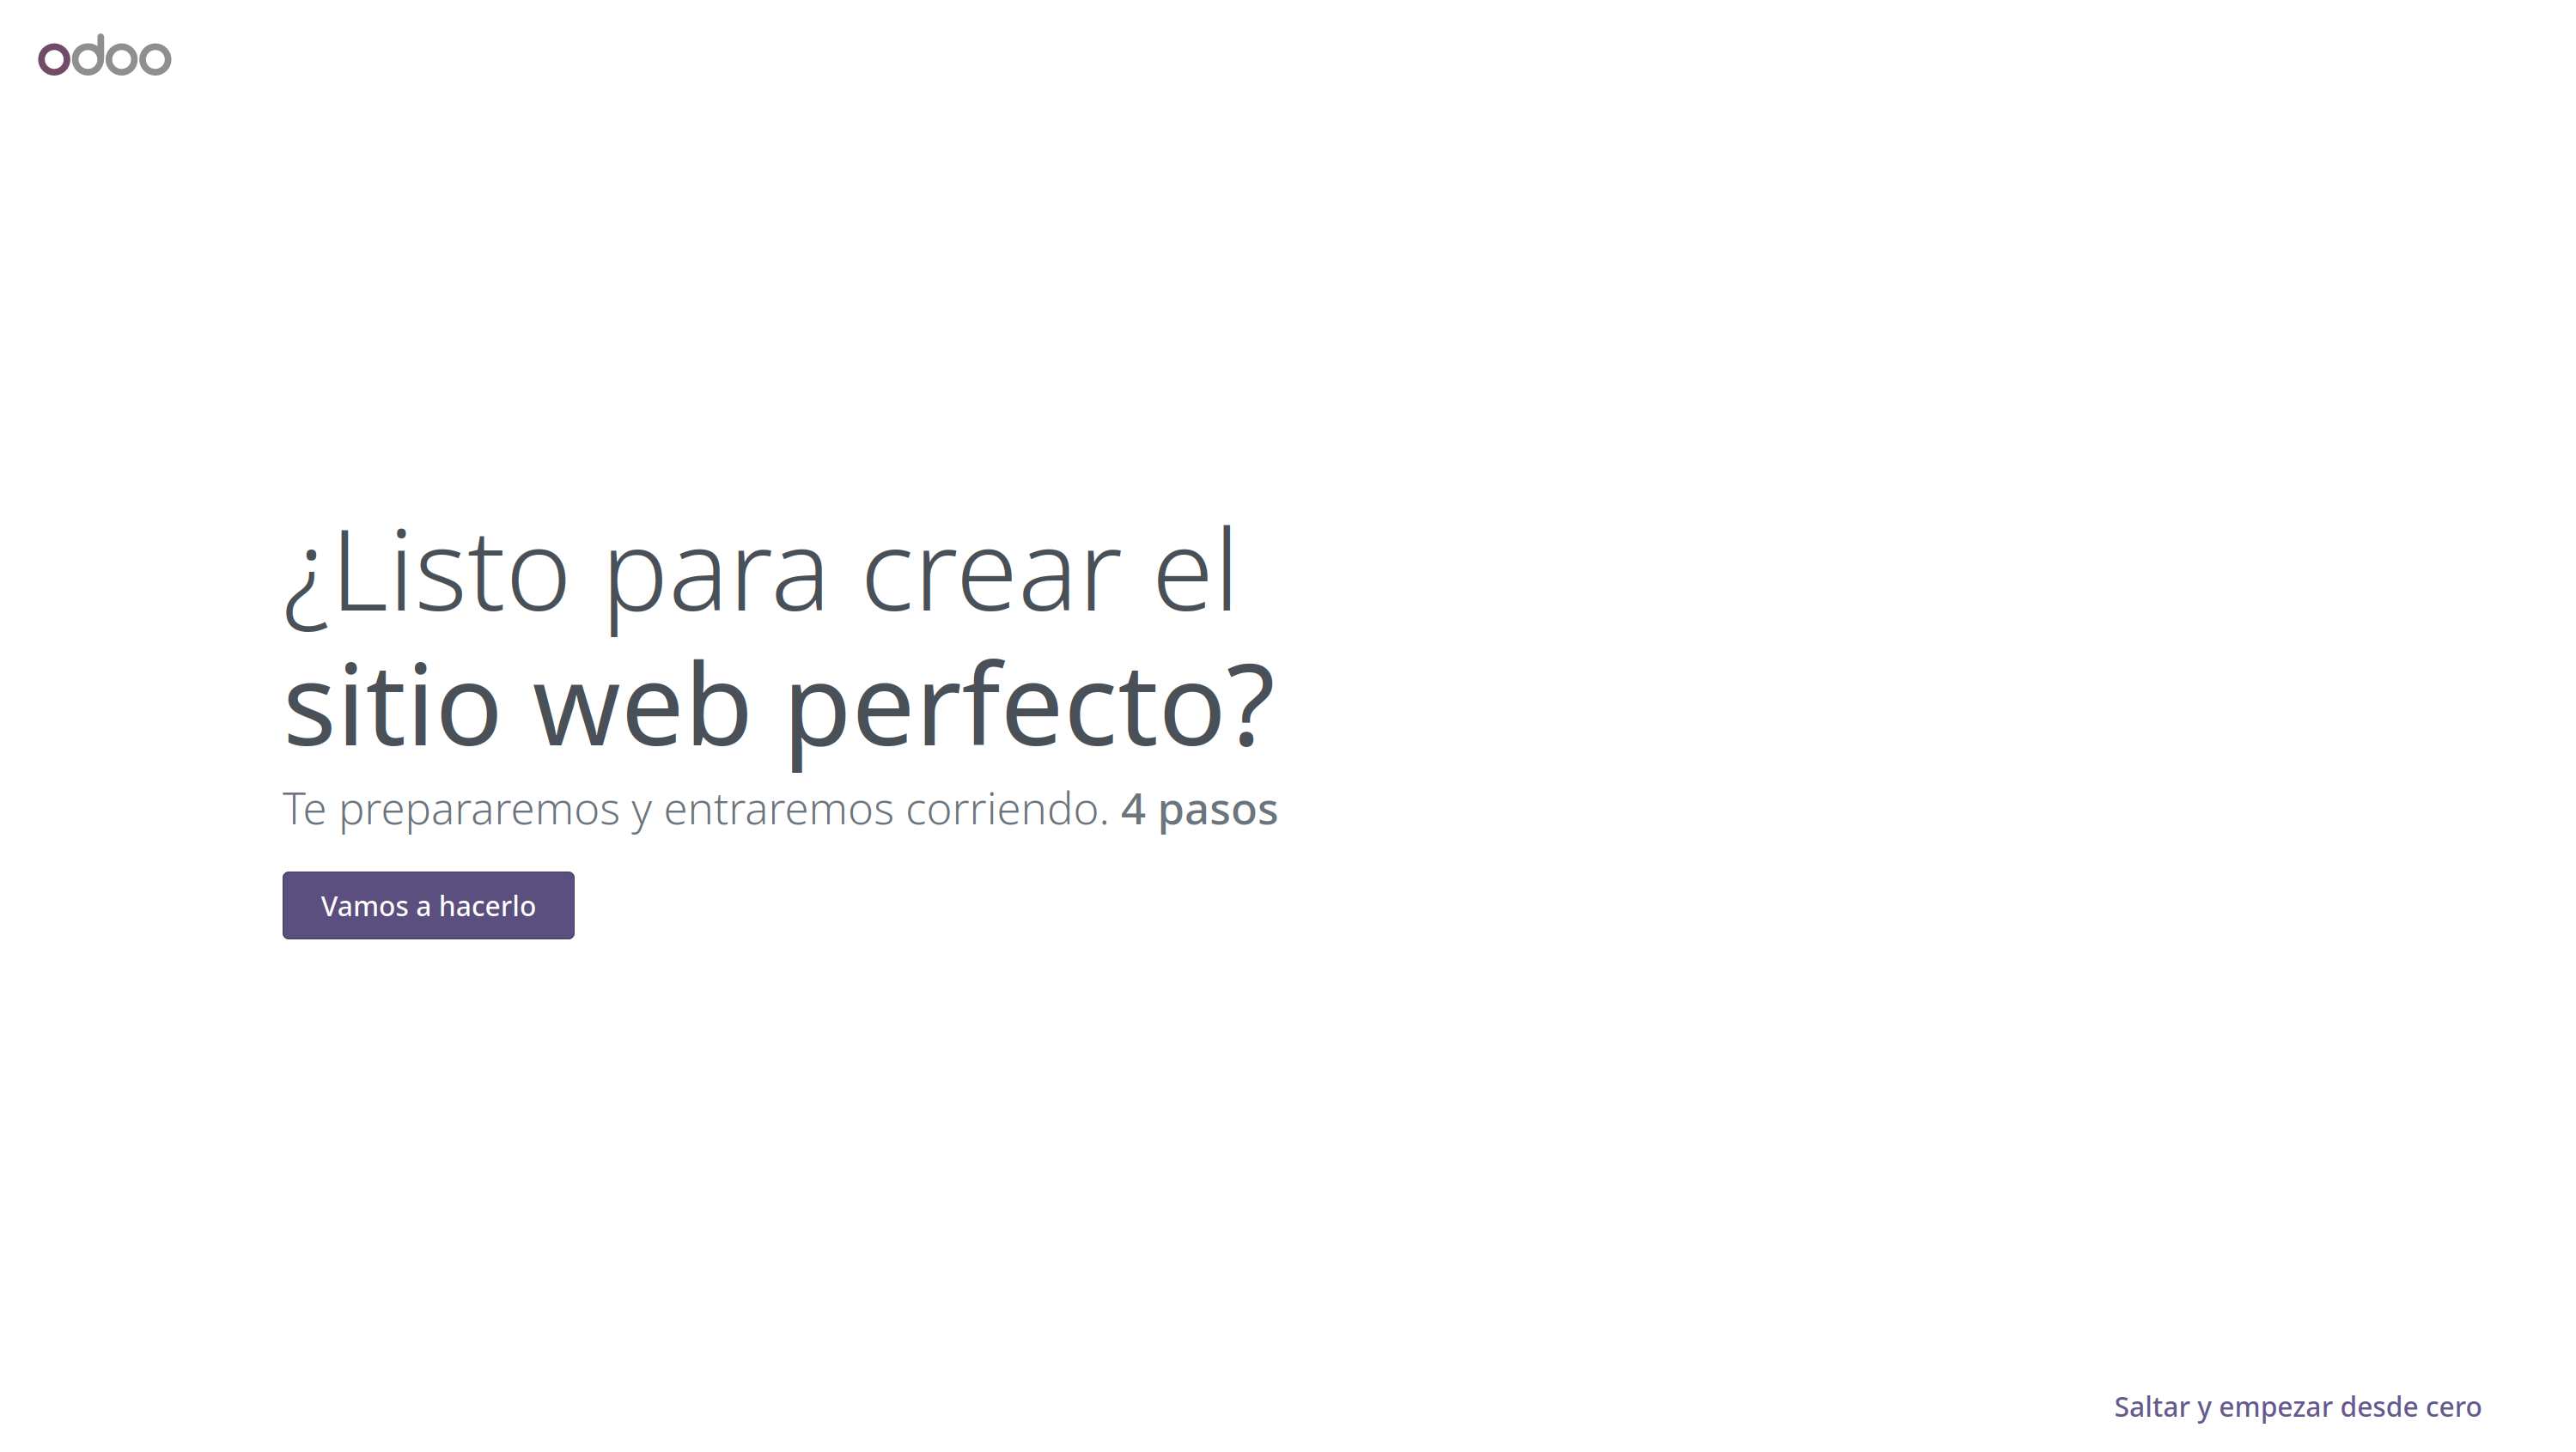
\includegraphics[width=6cm]{tutorial.png}
    \caption{Creación de la web}
    \label{fig:tutorial}
\end{figure}
En este menú se seleccionará la opción de Vamos a hacerlo, que permitirá crear la web de forma sencilla en 4 pasos. Selecciona e introduce la información que más se adecua al caso en particular y personaliza los colores y las características que tendrá la web. A continuación, se creará la web siguiendo la información enviada y se mostrará, en este caso se ha creado una web de alquiler de coches:
\begin{figure}[h]
    \centering
    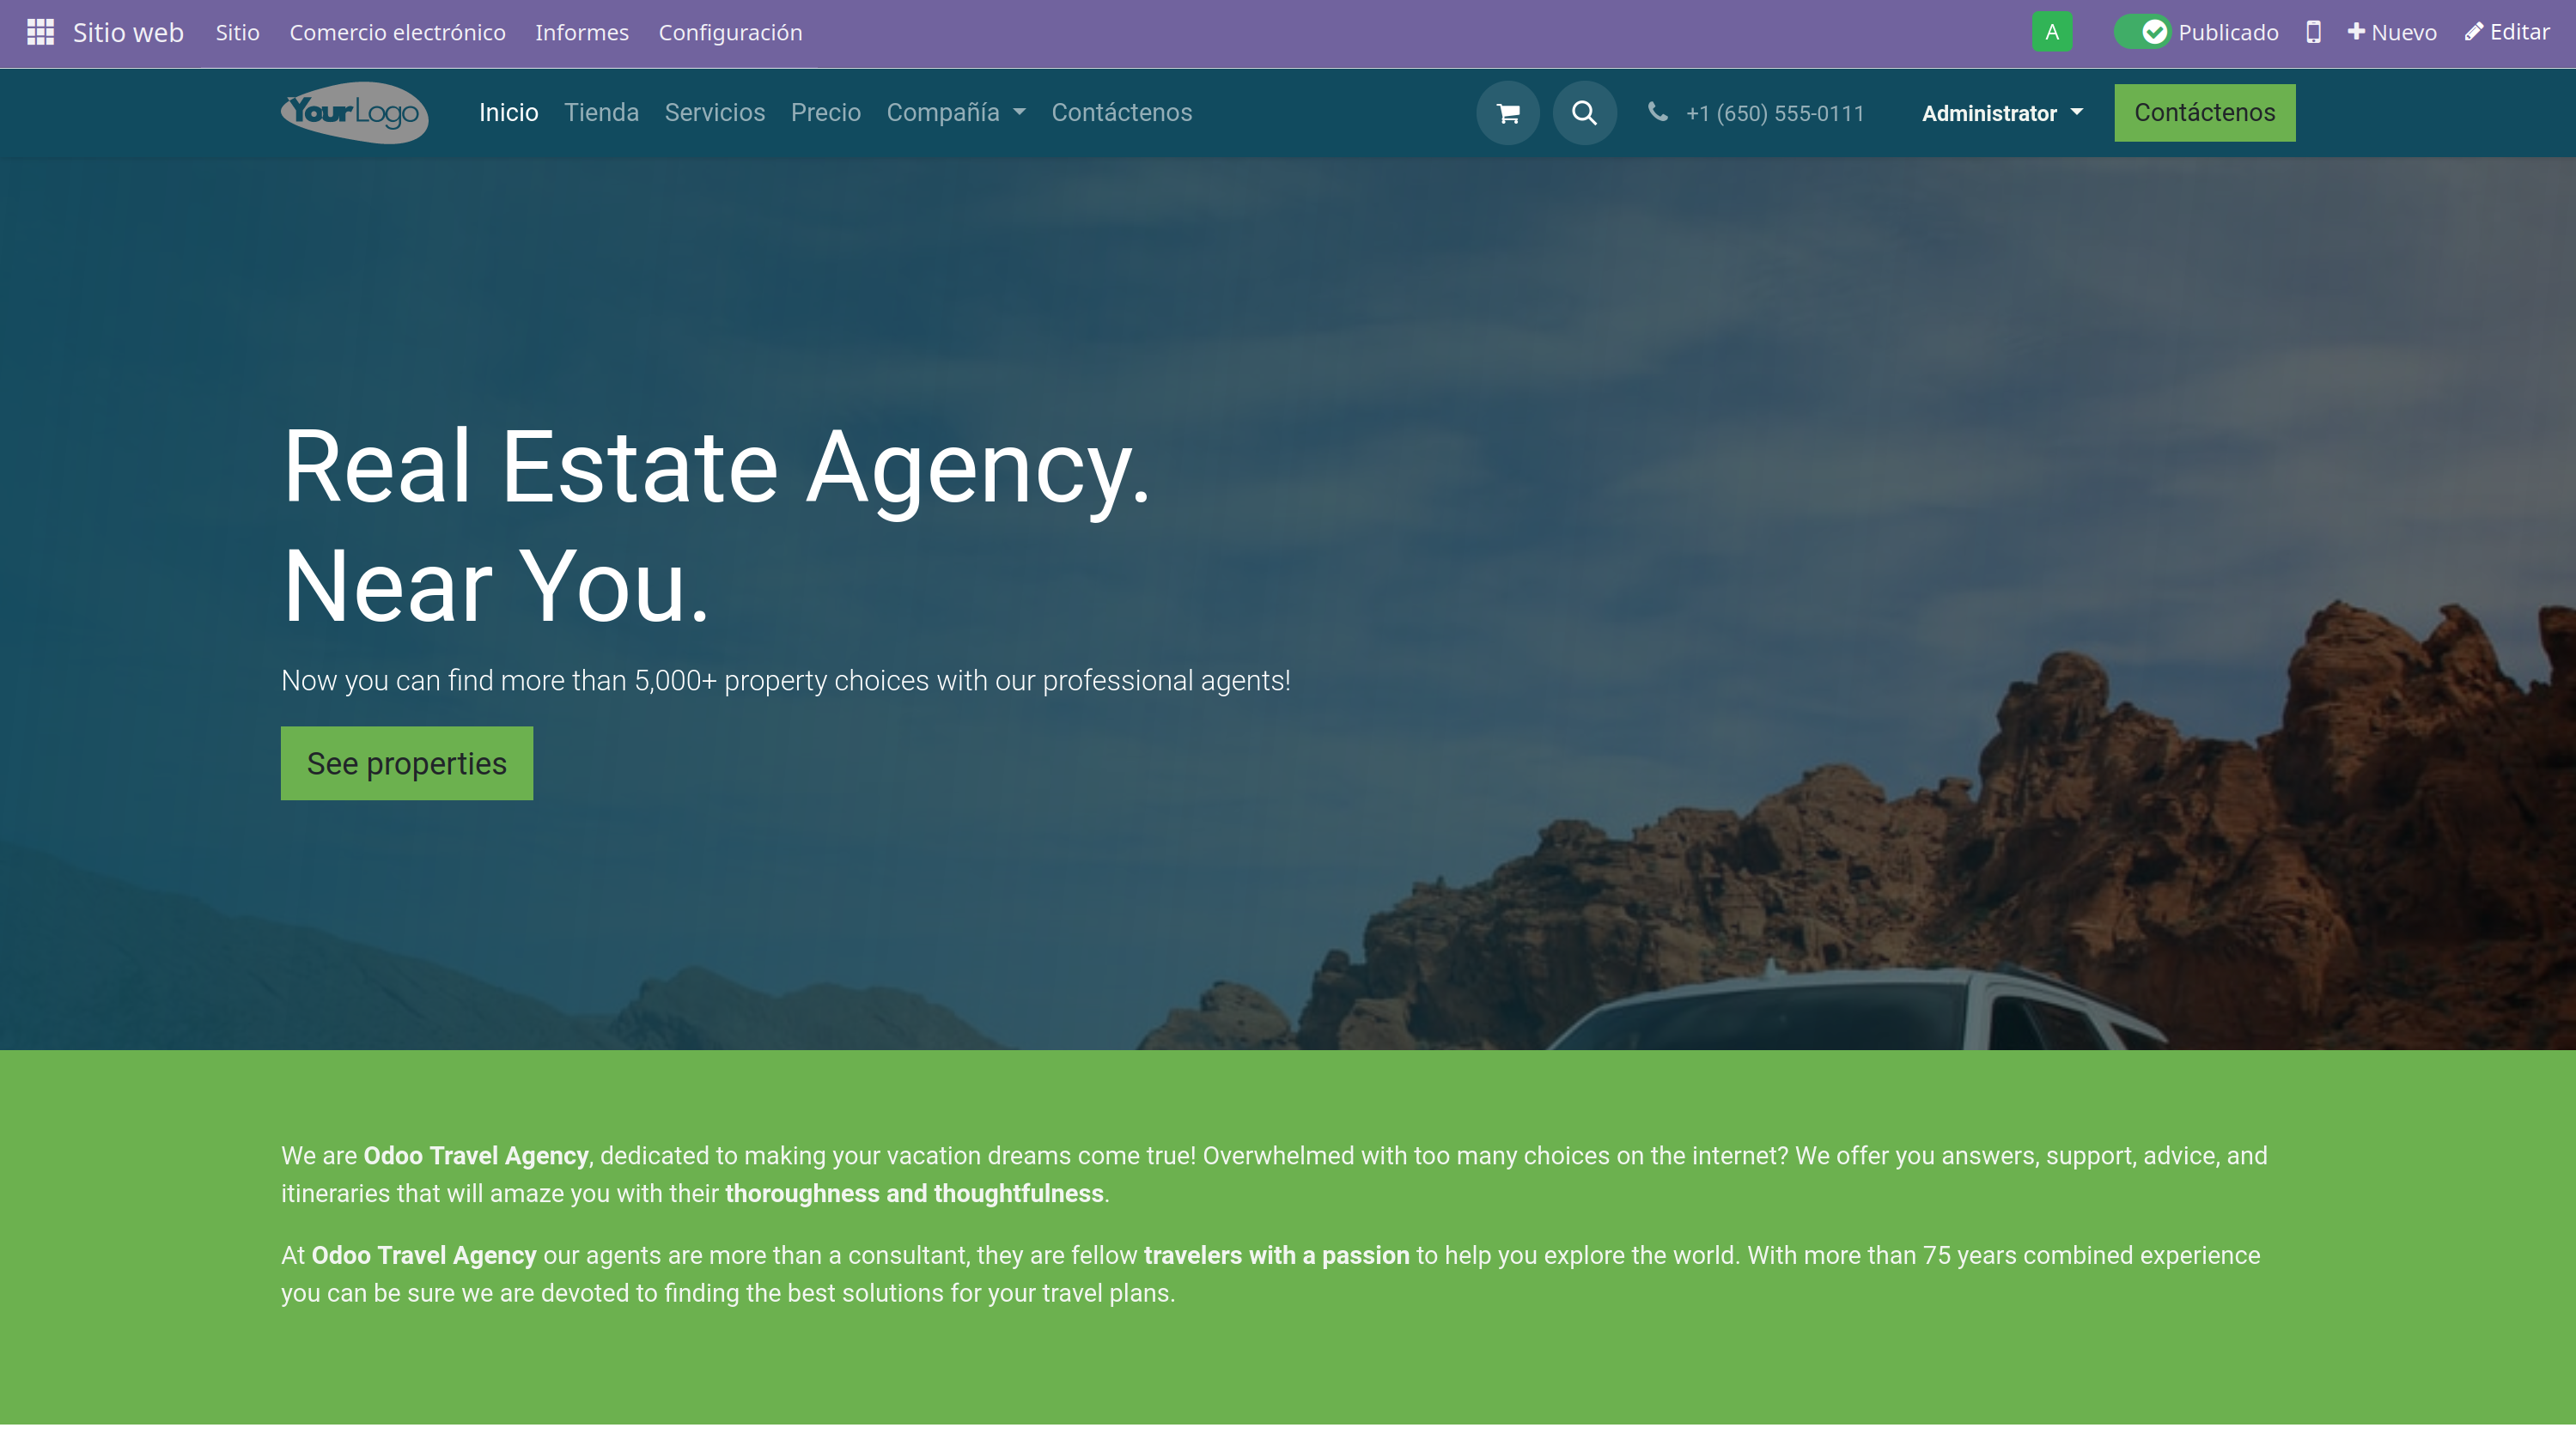
\includegraphics[width=6cm]{web.png}
    \caption{Sitio web creado automáticamente}
    \label{fig:web}
\end{figure}
Haz click en la opción Nuevo de la esquina superior derecha y selecciona Entrada de blog. Selecciona un blog existente o crea uno nuevo. Introduce el titulo de la entrada de blog y pulse guardar. Se mostrará la entrada de blog creada y un menú donde editar esta vista.
\paragraph{}
Si se clicka en el fondo verde que engloba el titulo se puede editar y añadir una imagen al fondo. Además, si se quiere añadir una galeria de fotos sobre el producto, en este caso el coche:
\begin{figure}[h]
    \centering
    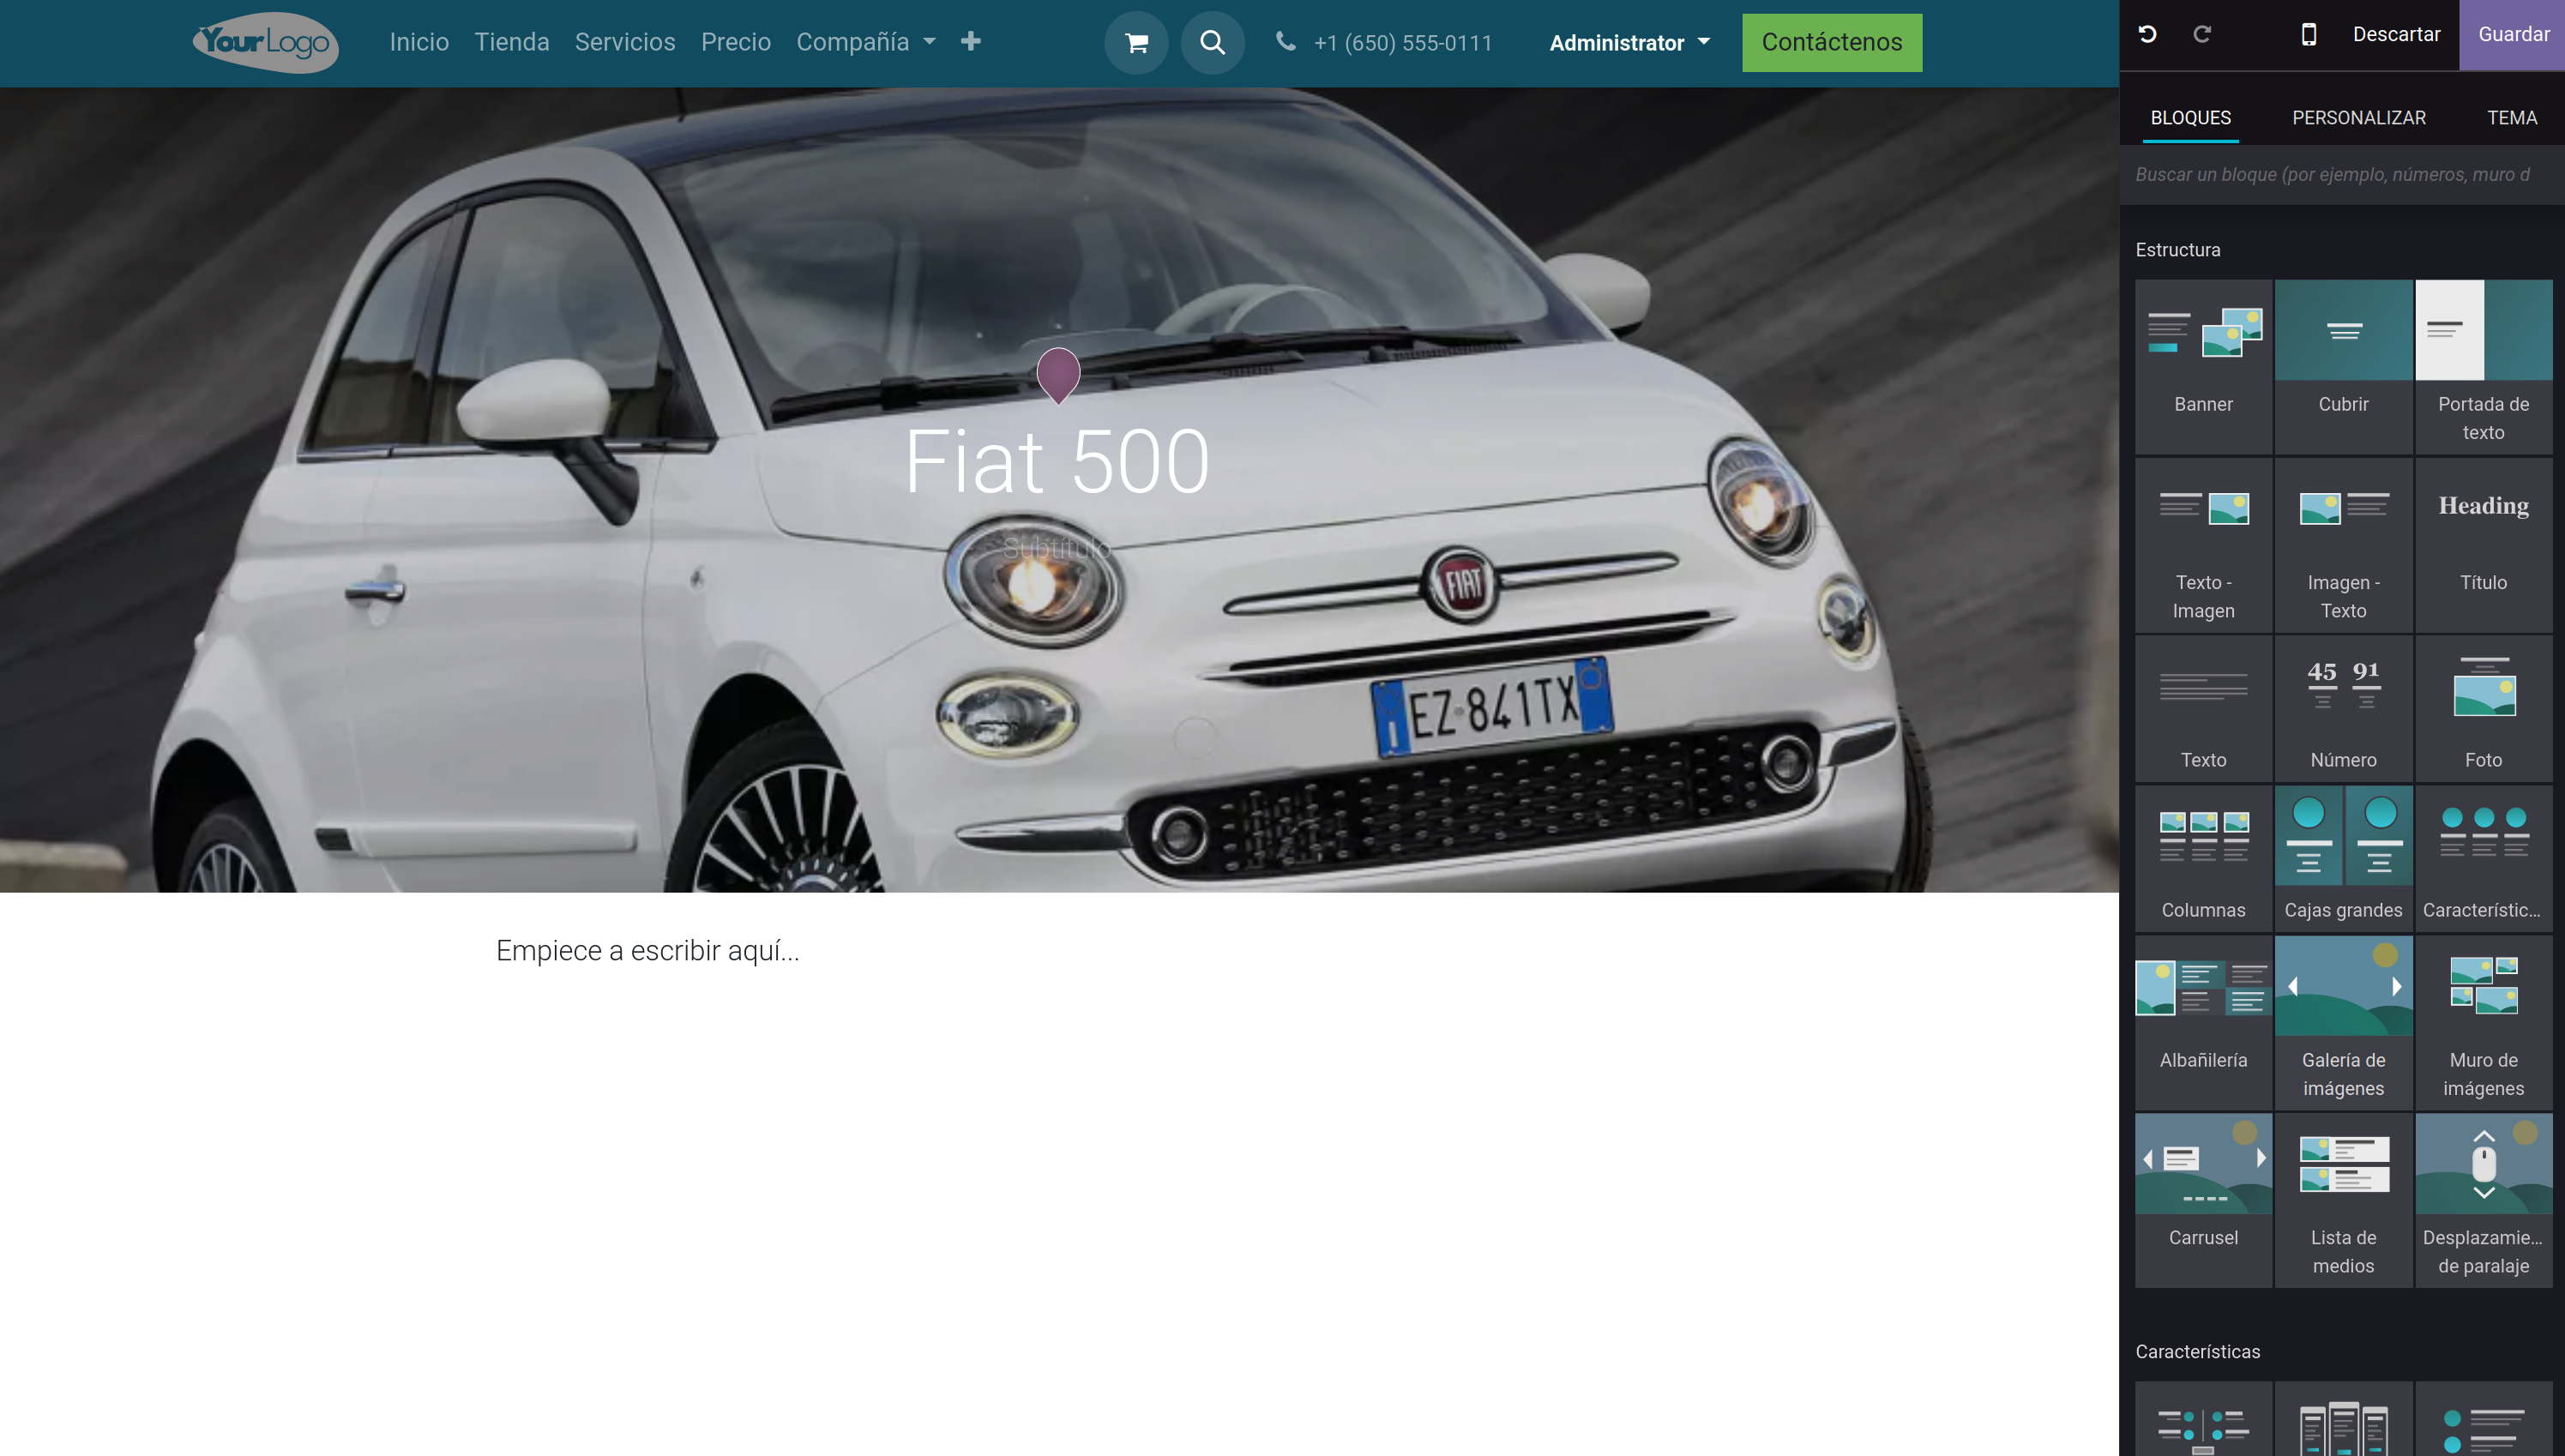
\includegraphics[width=6cm]{galeria.png}
    \caption{Adición de galería de fotos a la entrada de blog}
    \label{fig:galeria}
\end{figure}
Arrastra la galeria de imágenes del menú lateral derecho de edición y sueltalo en la parte de la web donde se quiere ubicar. Si haces click en la galeria, se mostrará un menu de edición en el lateral derecho donde se puede editar y personalizar. Para añadir las imagenes que se quieren mostrar se tendrá que dar click en Añadir en la opción de Imagenes dentro de la sección Galeria de imagenes del menú de edición. A continuación, hacer click en subir archivo y seleccionar las imagenes. Una vez subidas las fotos a Odoo, se hacer click en cada imagen de la galeria y se seleccionará la foto a mostrar. 
\paragraph{}
Si se quiere dar acceso a compra del producto mostrado se añadirá un bloque llamado Llamamiento a la acción de la misma manera que se ha hecho la galería de imágenes. Además, se puede editar cualquier texto de la web, para adecuar la información a las necesidades.
\begin{figure}[h]
    \centering
    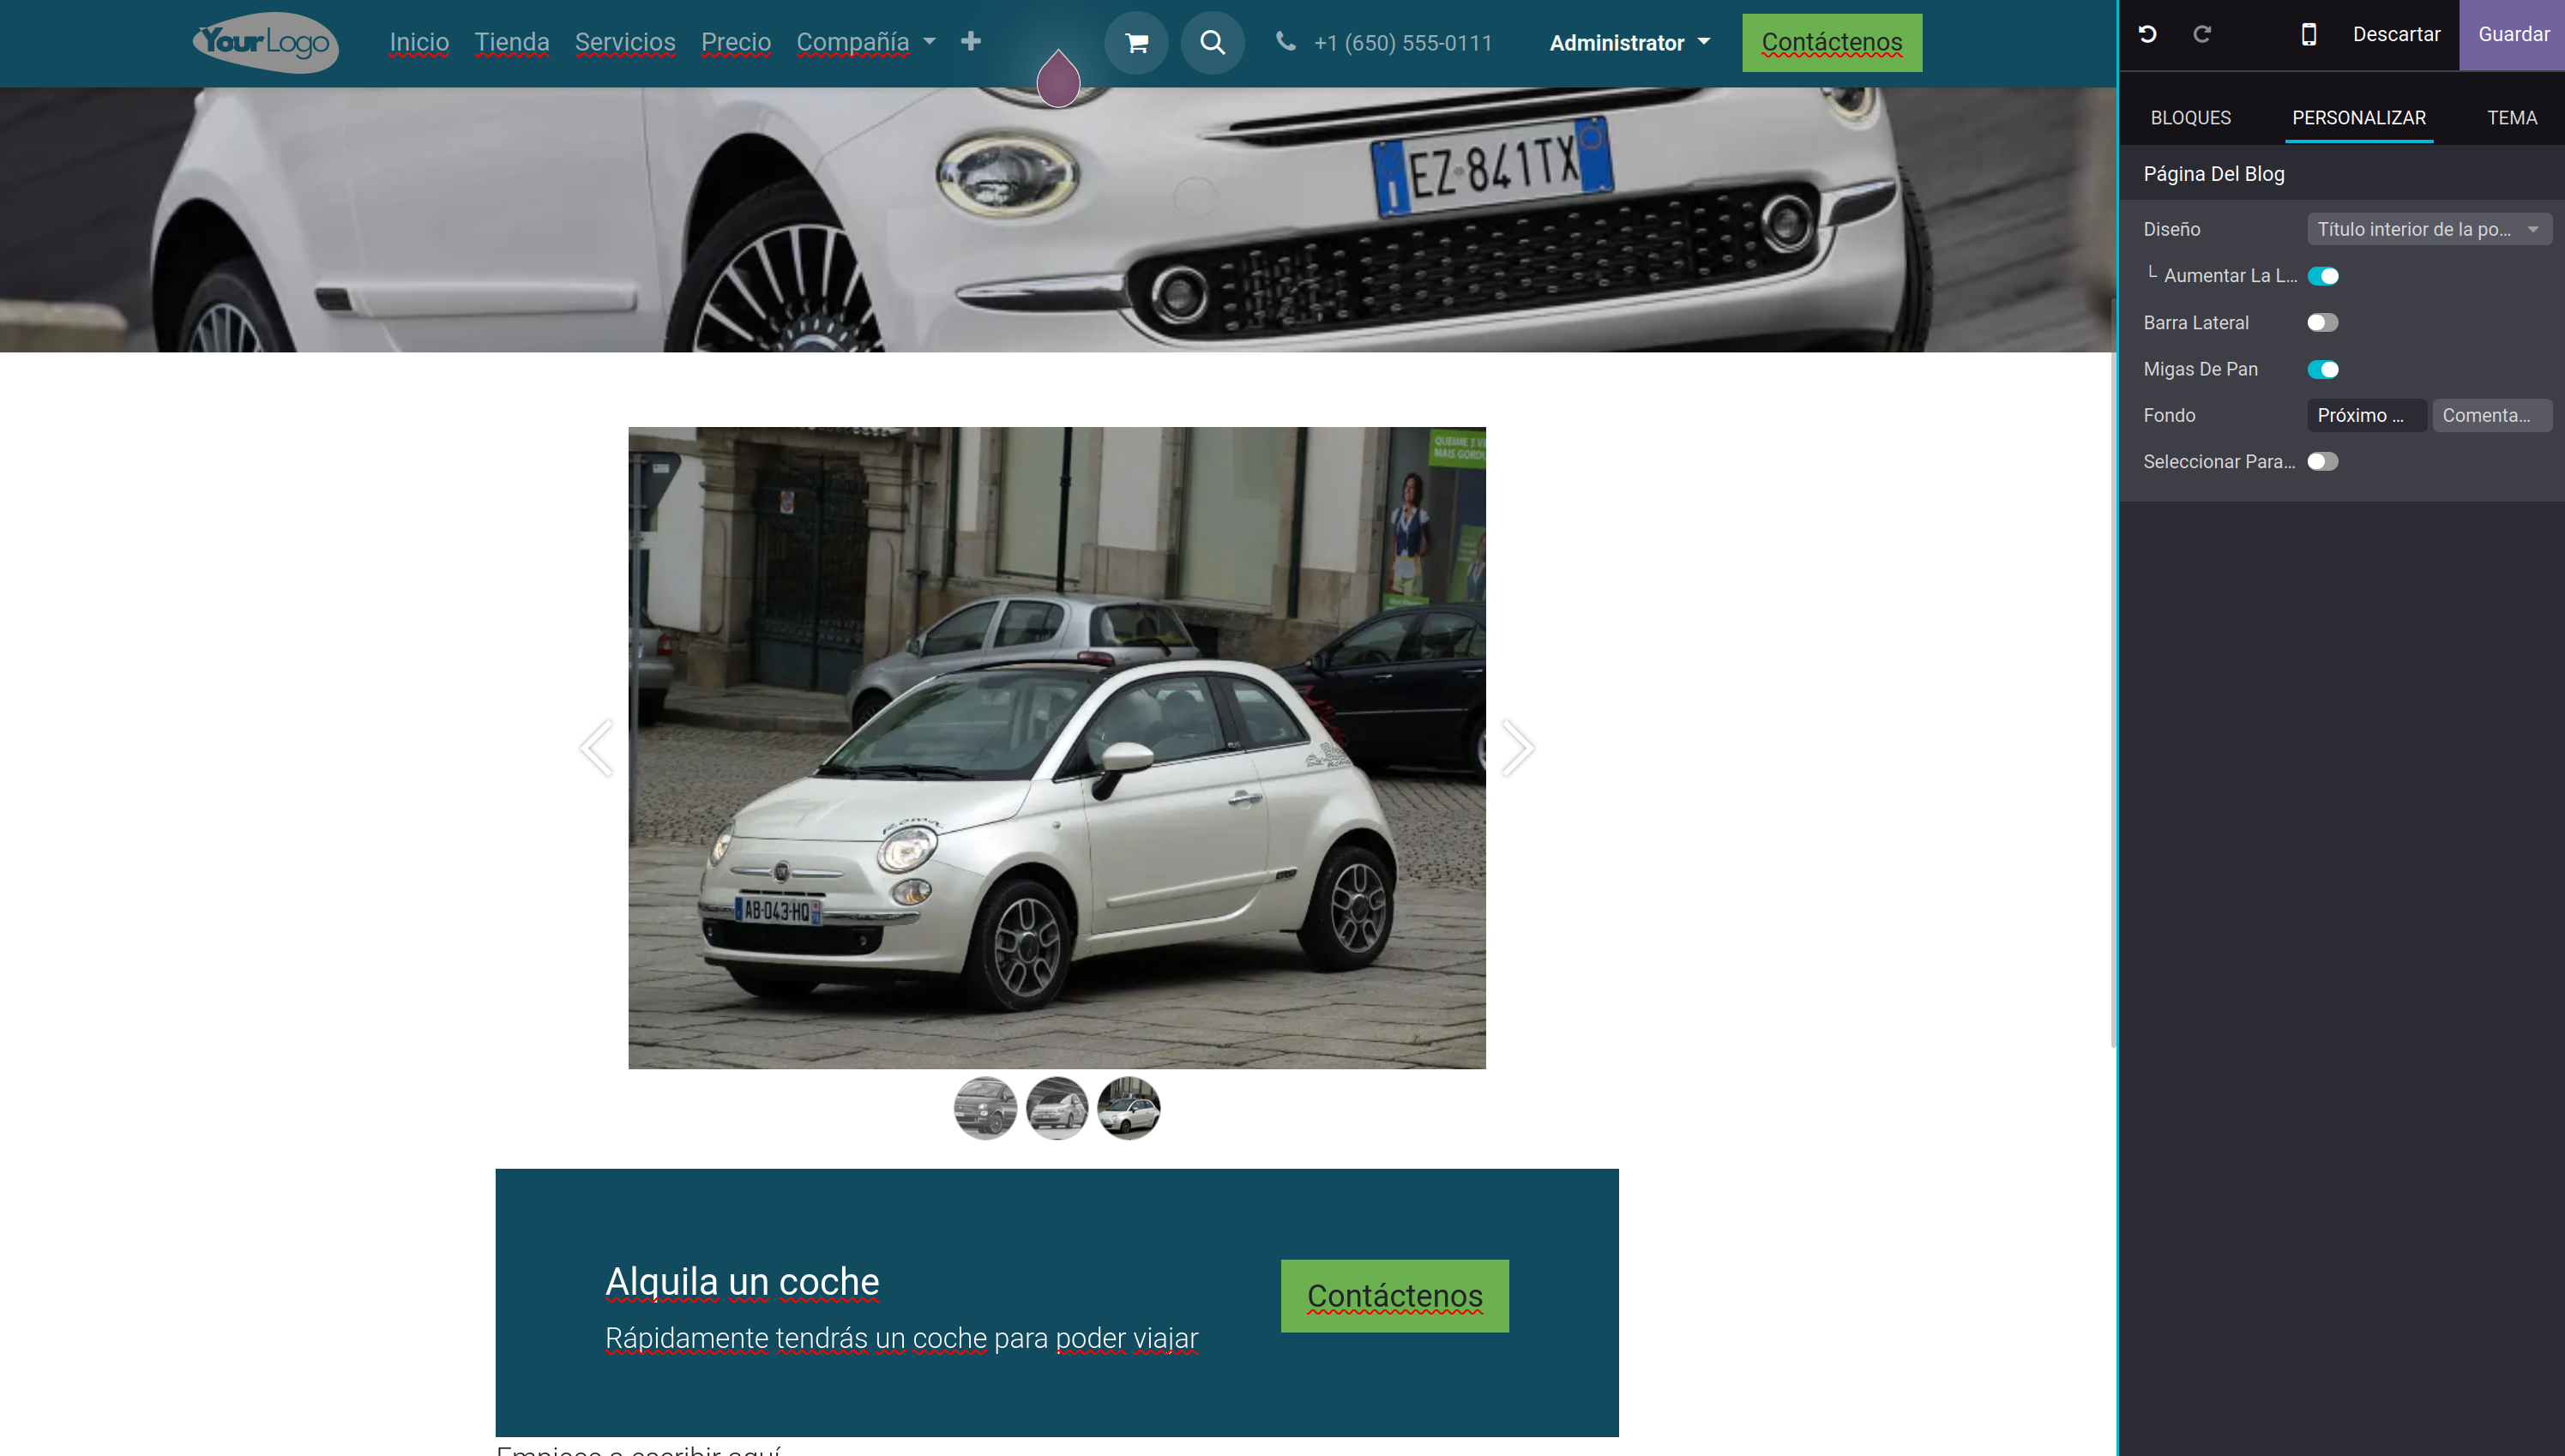
\includegraphics[width=6cm]{callToAction.png}
    \caption{Adición de un llamamiento a la acción a la entrada de blog}
    \label{fig:callToAction}
\end{figure}
Una vez, la entrada de blog esté a su gusto guárdalo clickando en el botón guardar de la esquina superior derecha.
\paragraph{}
Para añadir una página nueva al sitio web añadimos una página como en la figura 4. Selecciona la opción Servicios del menu lateral izquierdo y elige la página que más se adecua a las necesidades, en este caso se va a crear un sitio donde están las preguntas frecuentes, problemas comunes y sus soluciones, por lo que se va a elegir la segunda opción.
\begin{figure}[h]
    \centering
    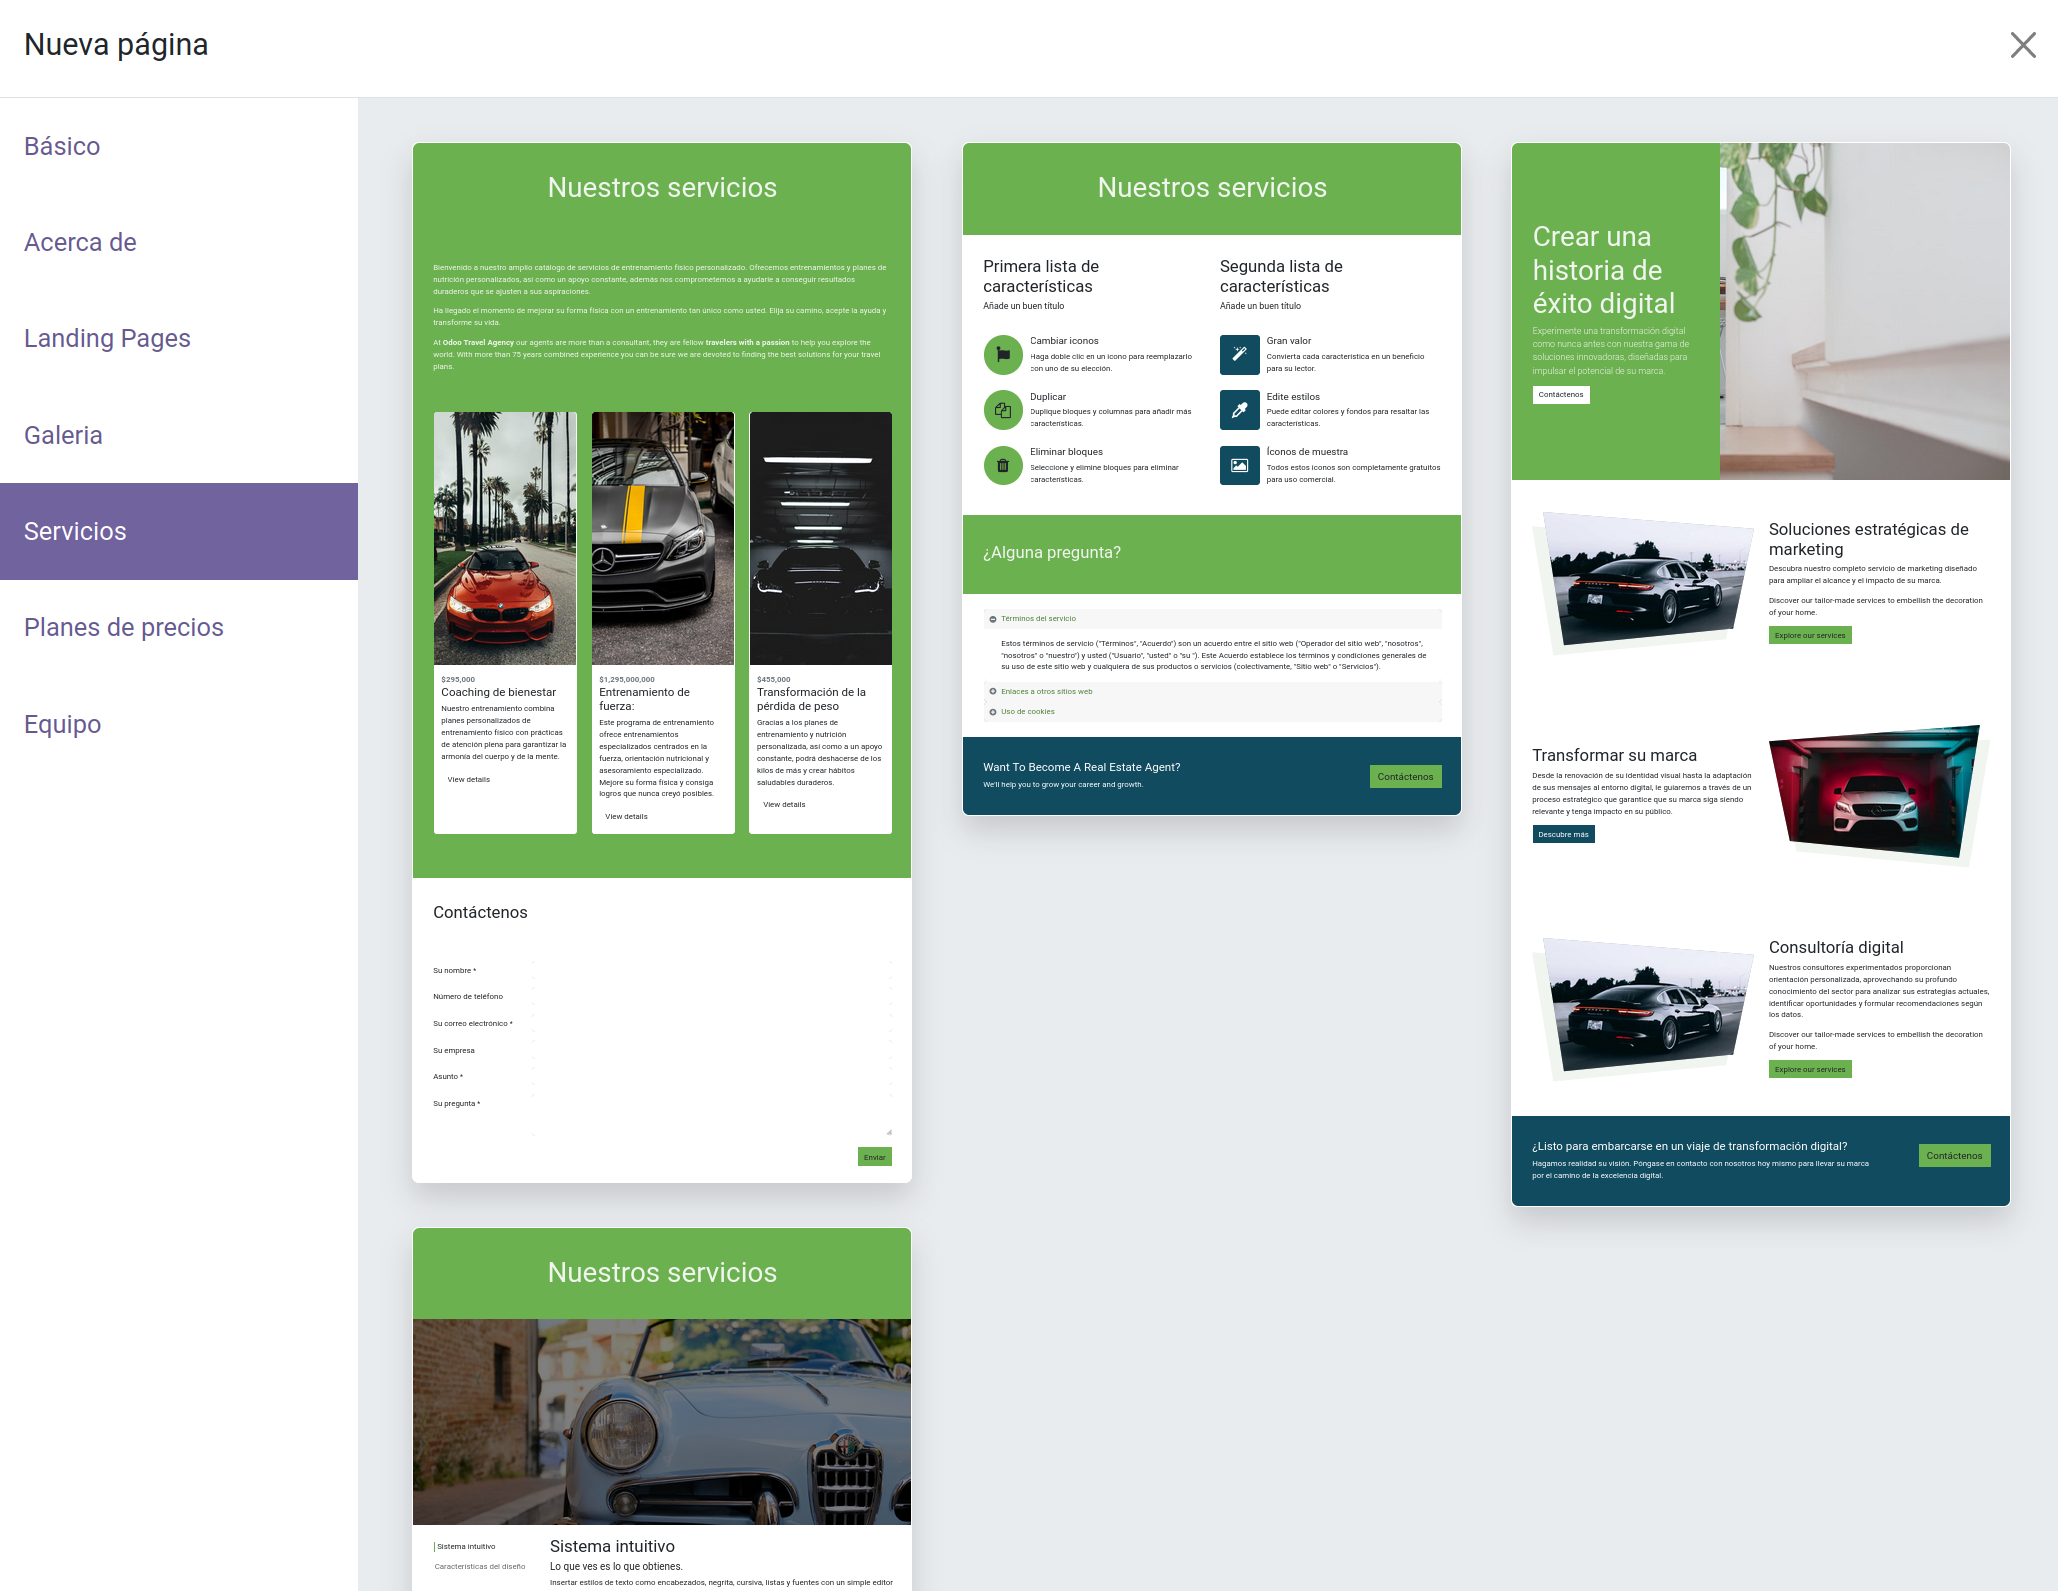
\includegraphics[width=6cm]{addPagina.png}
    \caption{Creación de una página para mostrar FAQs}
    \label{fig:addPagina}
\end{figure}
Introduce el titulo de la página, deja activada la opción de Añadir al menú y pulsa en crear.
\begin{figure}[h]
    \centering
    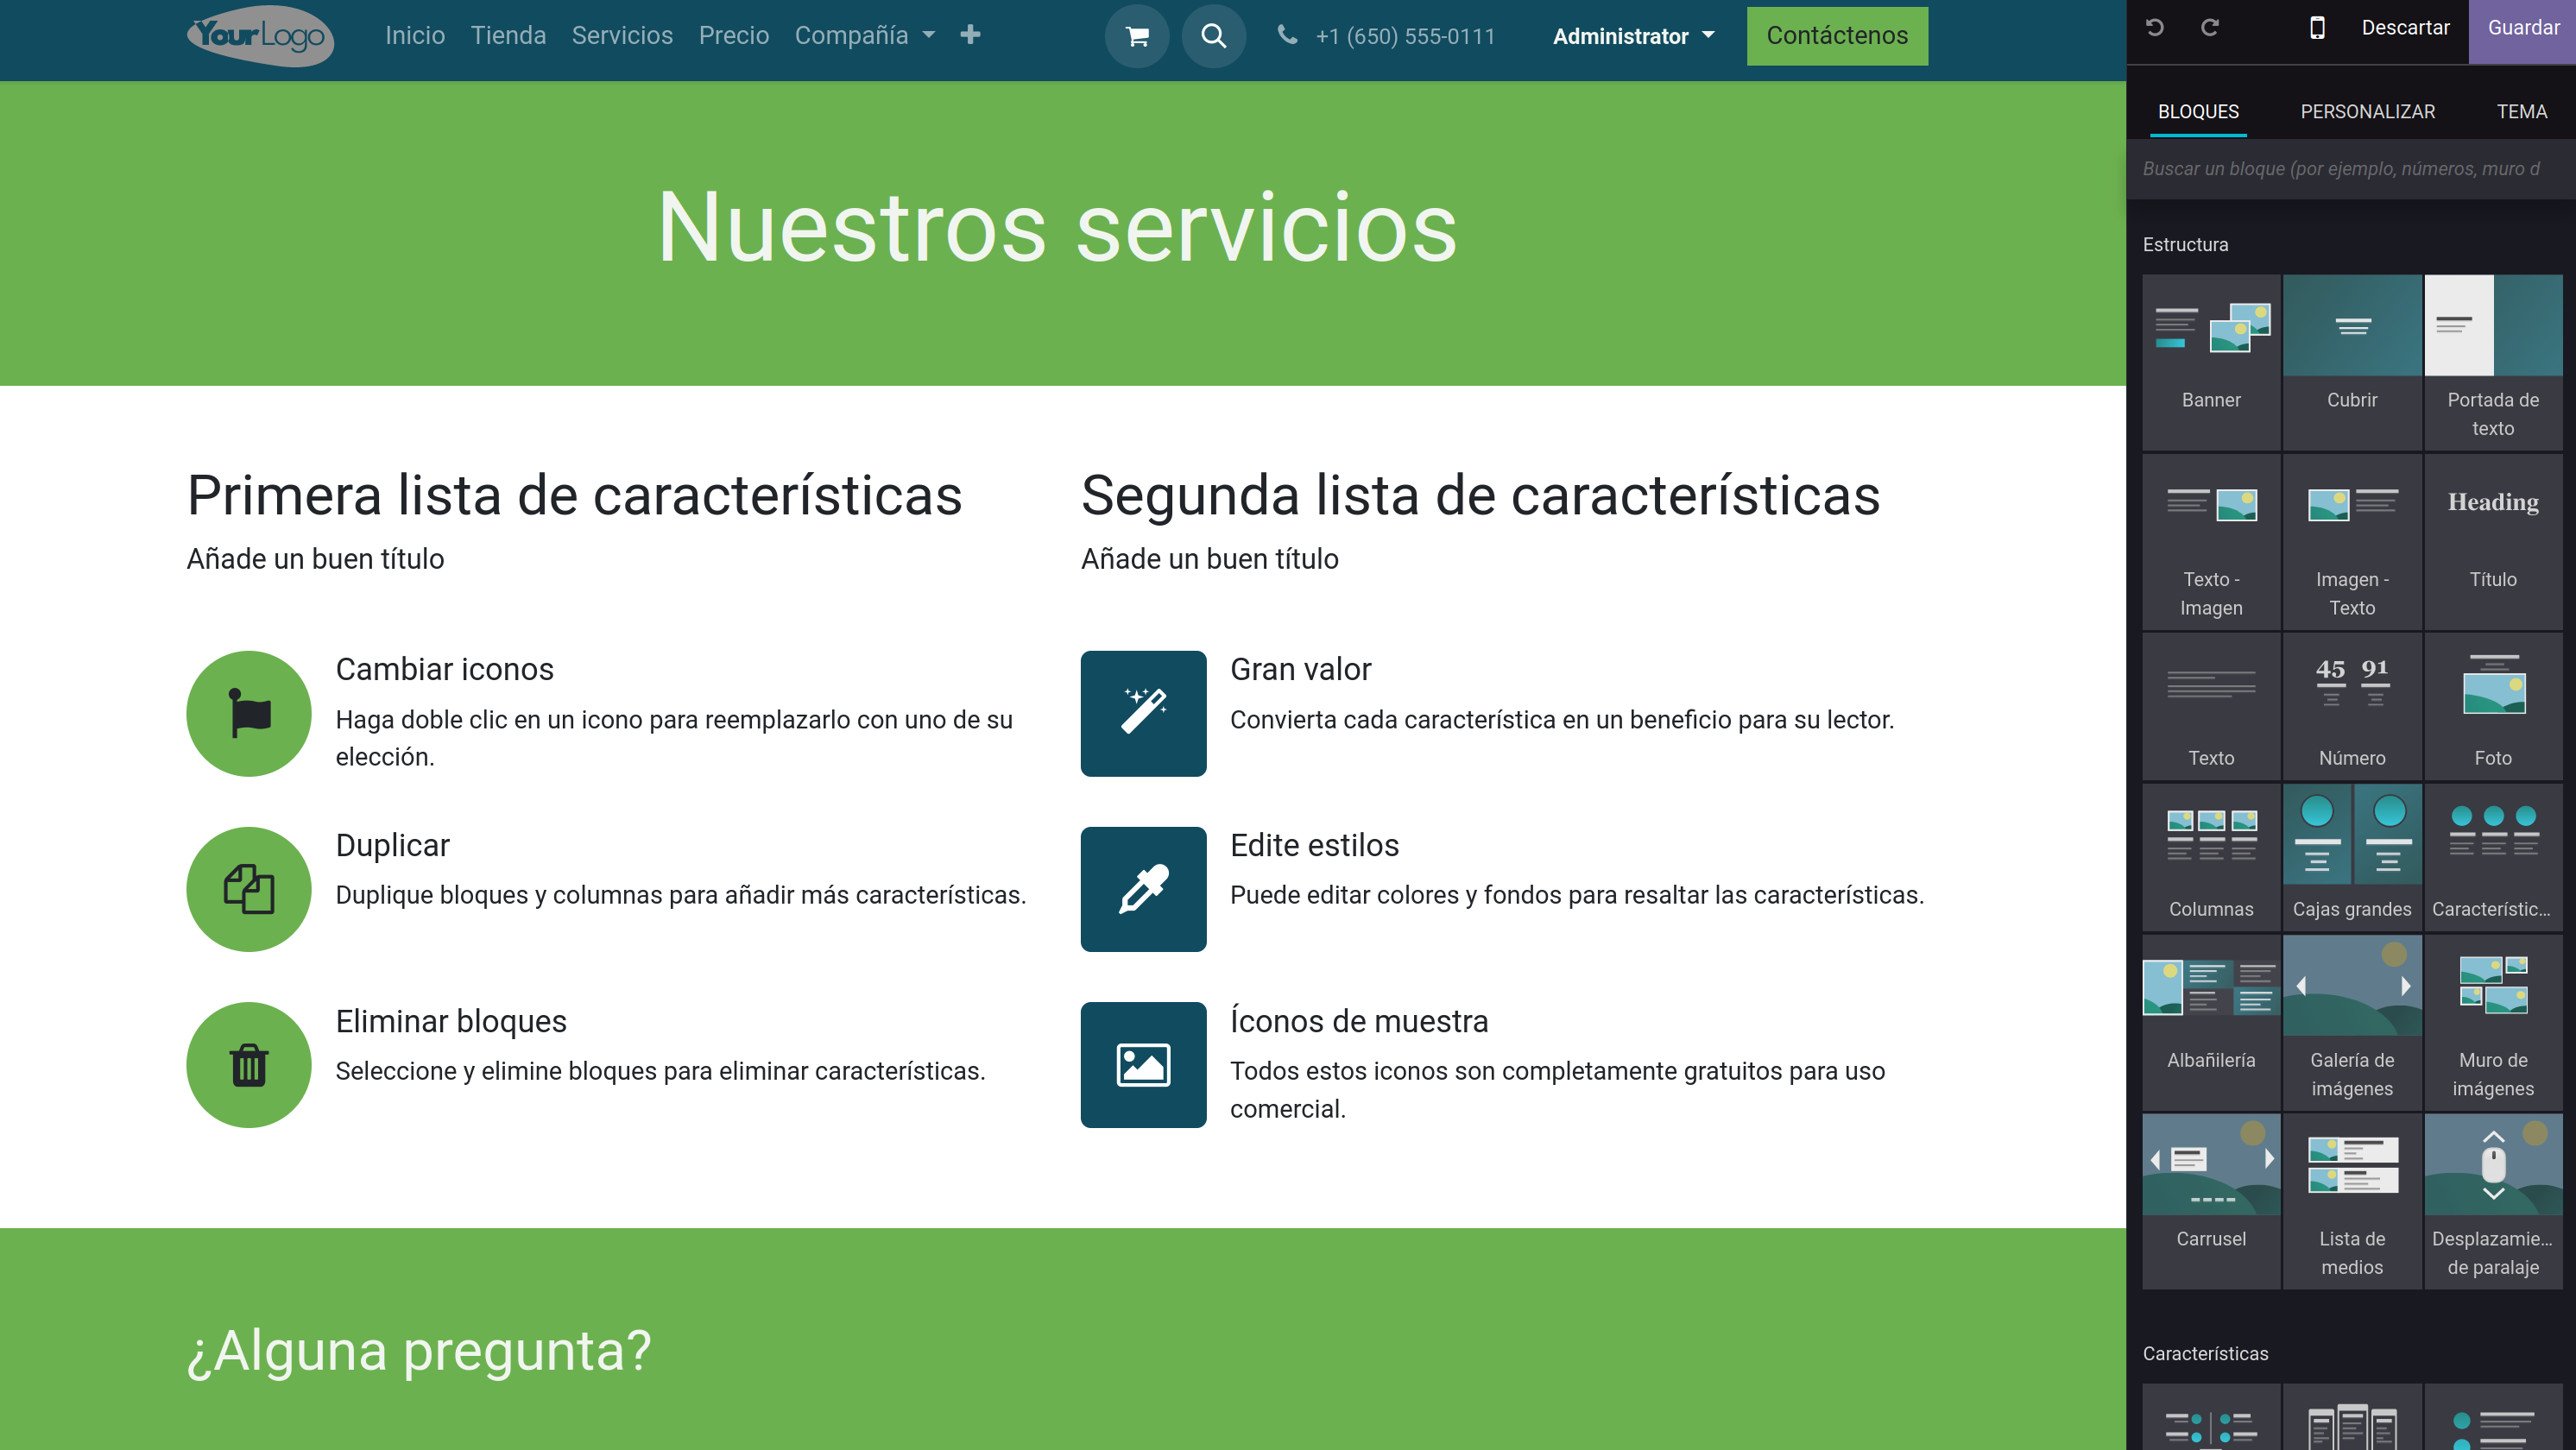
\includegraphics[width=6cm]{paginaNueva.png}
    \caption{Página para mostrar FAQs creada}
    \label{fig:paginaNueva}
\end{figure}
Como ya hemos explicado anteriormente, edita y personaliza cada texto y foto para que se ajuste a las necesidades propias. Vamos a centrarnos en el contenido importante de esta página que son las preguntas y problemas frecuentes y como solucionarlo. Para ello, se va a utilizar el bloque acordeón que ya existe en la parte inferior de la página. Para añadir nuevos temas clica encima del acordeón y clica en Añadir Artículo de la opción Tema de la sección Acordeón del menú lateral derecho. Se añadirá un nuevo artículo al final del acordeón, selecciona cada texto para incluir la información personalizada y selecciona la opción junto a la basura, para arrastrar el artículo y ordenarlos dentro del acordeón.
\begin{figure}[h]
    \centering
    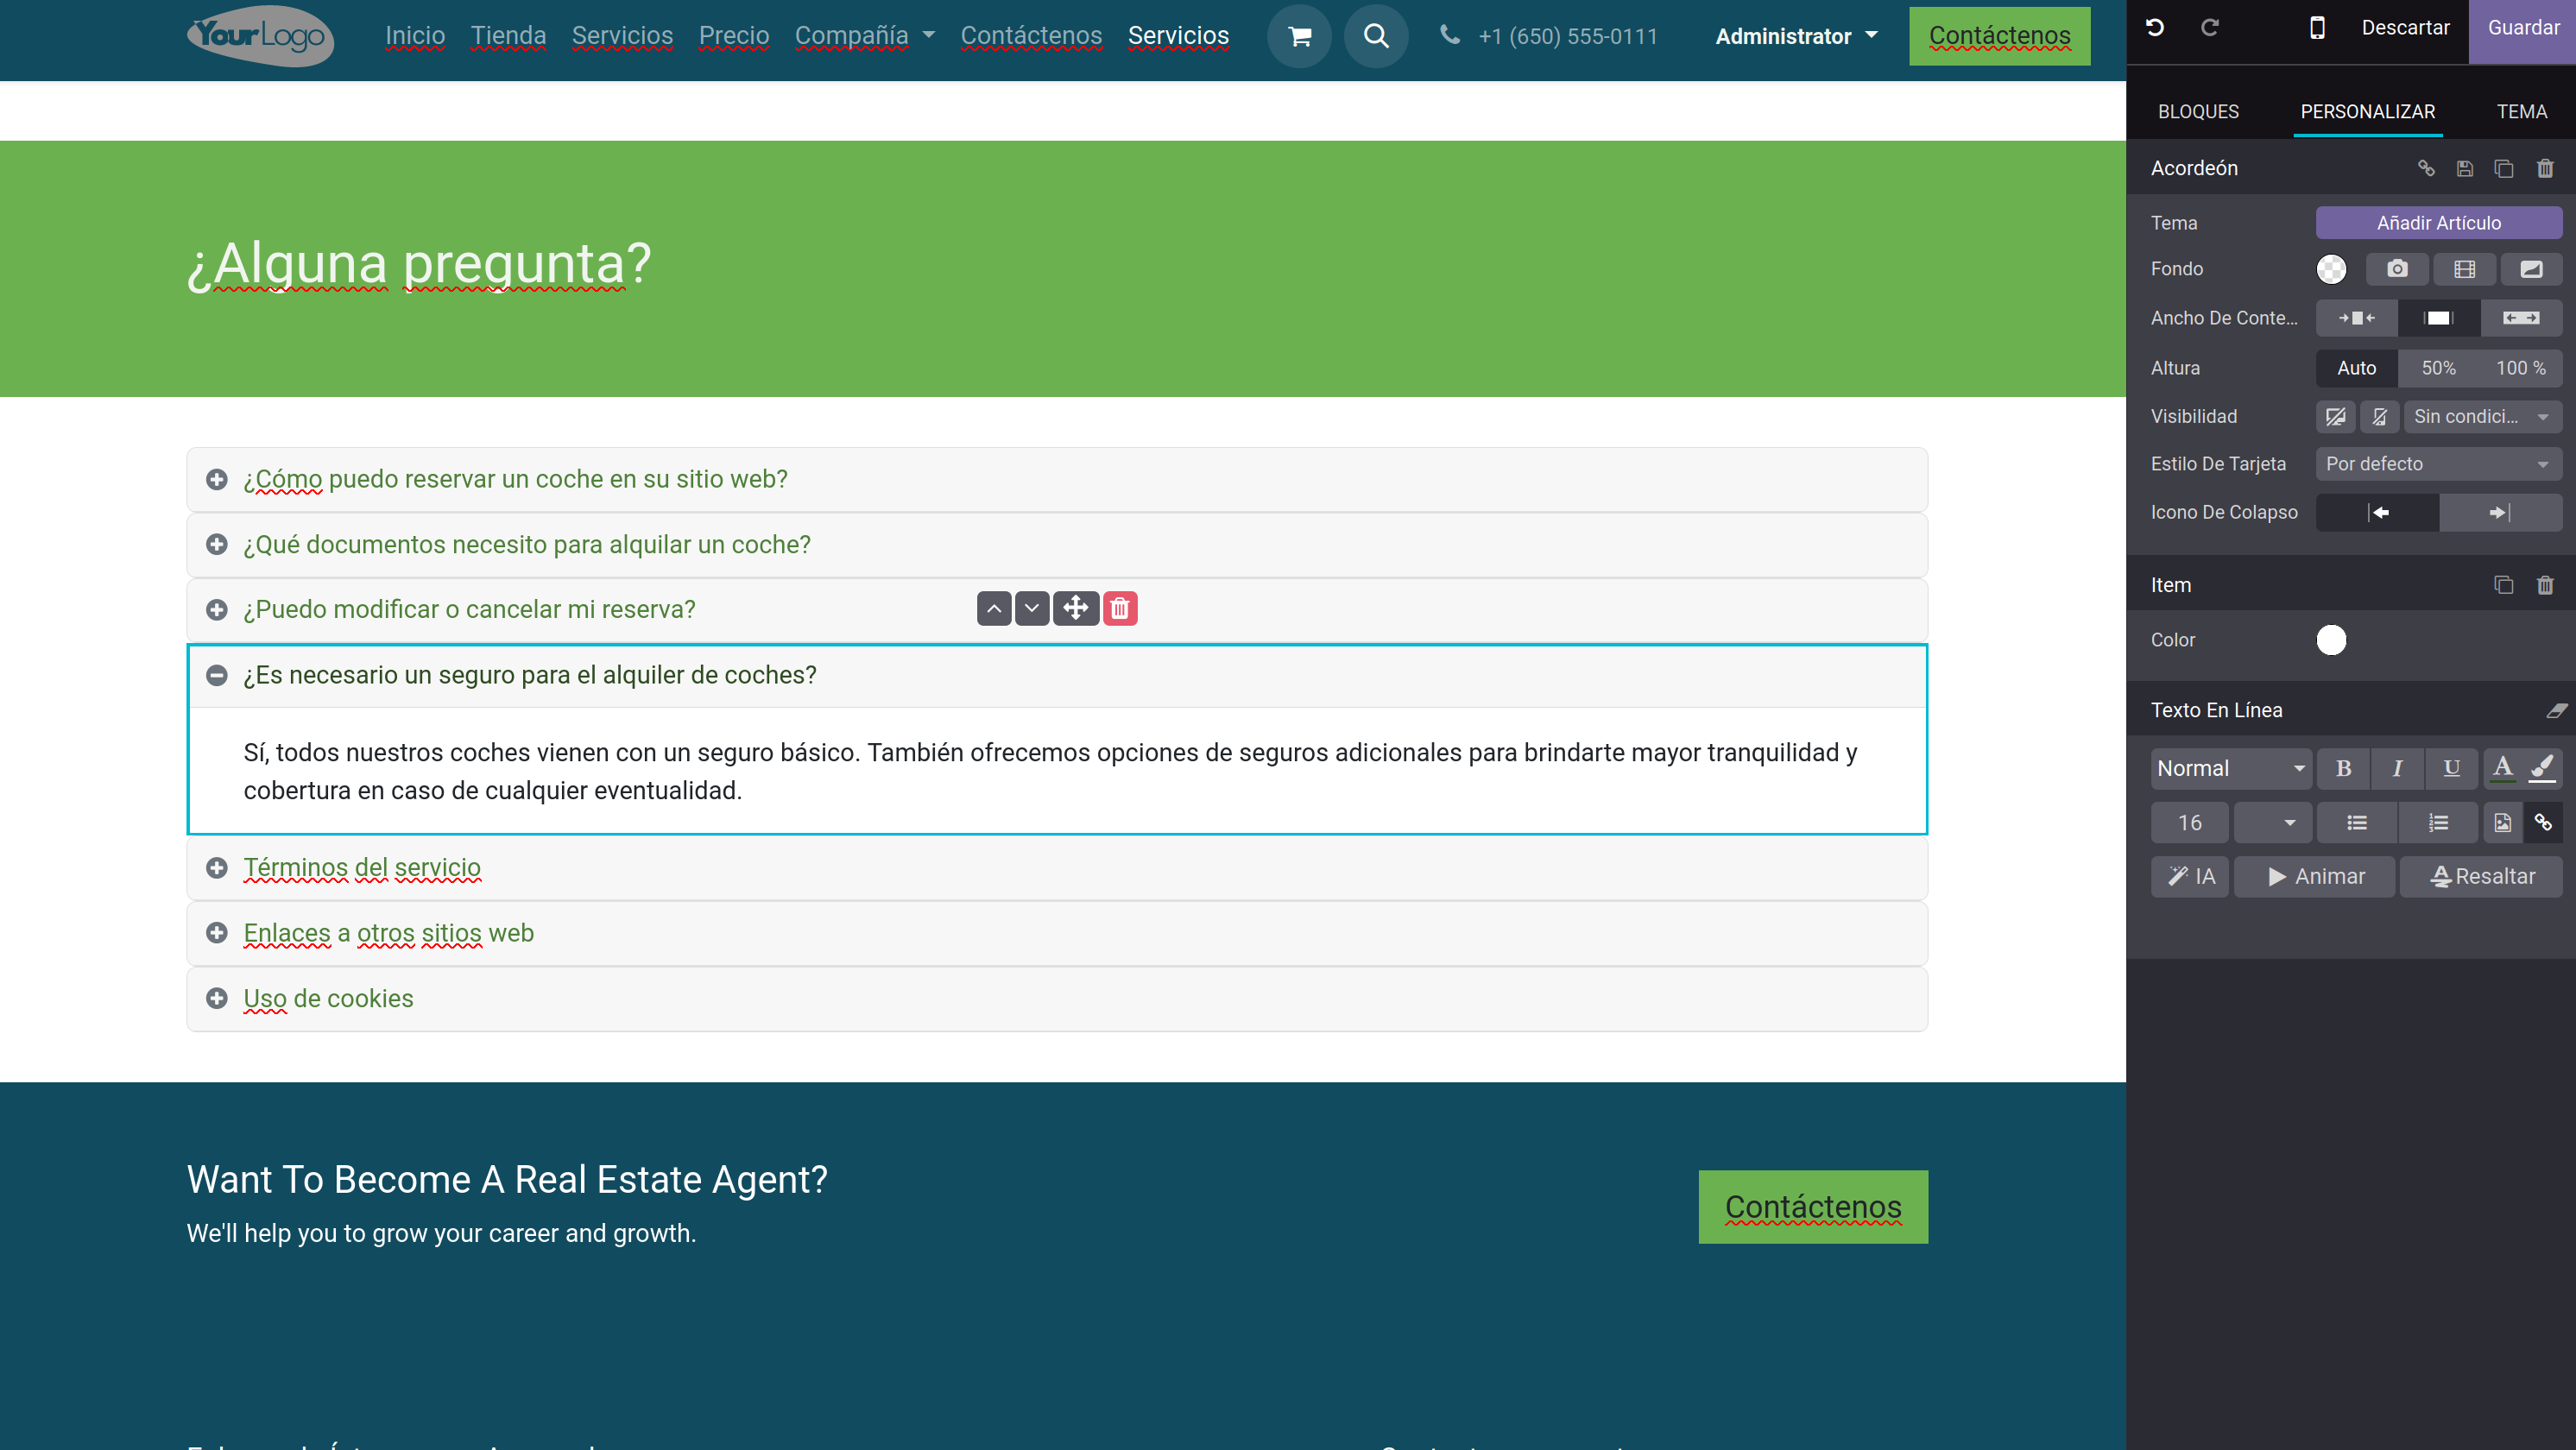
\includegraphics[width=6cm]{faqs.png}
    \caption{Creando el acordeón con los FAQs}
    \label{fig:faqs}
\end{figure}
Finalmente, haz click en guardar en la esquina superior derecha.
\section{Configuración}
\paragraph{}
A continuación, se va a llevar a cabo la configuración funcional de Odoo. Para ello se va a explicar paso a paso el proceso de creación de una compañía. Primero, se debe ir al menú de configuración dentro de las opciones generales. Se hace click en el link Administrar compañías.
\newpage
\begin{figure}[h]
    \centering
    \includegraphics[width=6cm]{adminCompañias.png}
    \caption{Página de configuración de opciones generales}
    \label{fig:faqs}
\end{figure}
Luego en la esquina superior izquierda selecciona el botón New. Se llegará al menú de creación de una compañía.
\begin{figure}[h]
    \centering
    \includegraphics[width=6cm]{crearCompañias.png}
    \caption{Creando una nueva compañía}
    \label{fig:faqs}
\end{figure}
\paragraph{}
Introduce los datos correspondientes a la compañía que se quiere crear. Por último, si navegas hacia atrás a la página de administración de las compañías verás que se ha creado una nueva. Además, si se quieren crear compañías en otros países que sean ramas de una compañía matriz, se debe seleccionar desde la página de administración de compañías la compañía que se quiere que sea la matriz. Se entra en el menú Ramas donde se puede administrar las compañías ramas. 
\begin{figure}[h]
    \centering
    \includegraphics[width=6cm]{ramasCompañias.png}
    \caption{Página de administración de compañías rama.}
    \label{fig:faqs}
\end{figure}
\paragraph{}
Para crear una compañía rama pulsa en la opción Agregar línea y rellena la información correspondiente. 
\newpage
\begin{figure}[h]
    \centering
    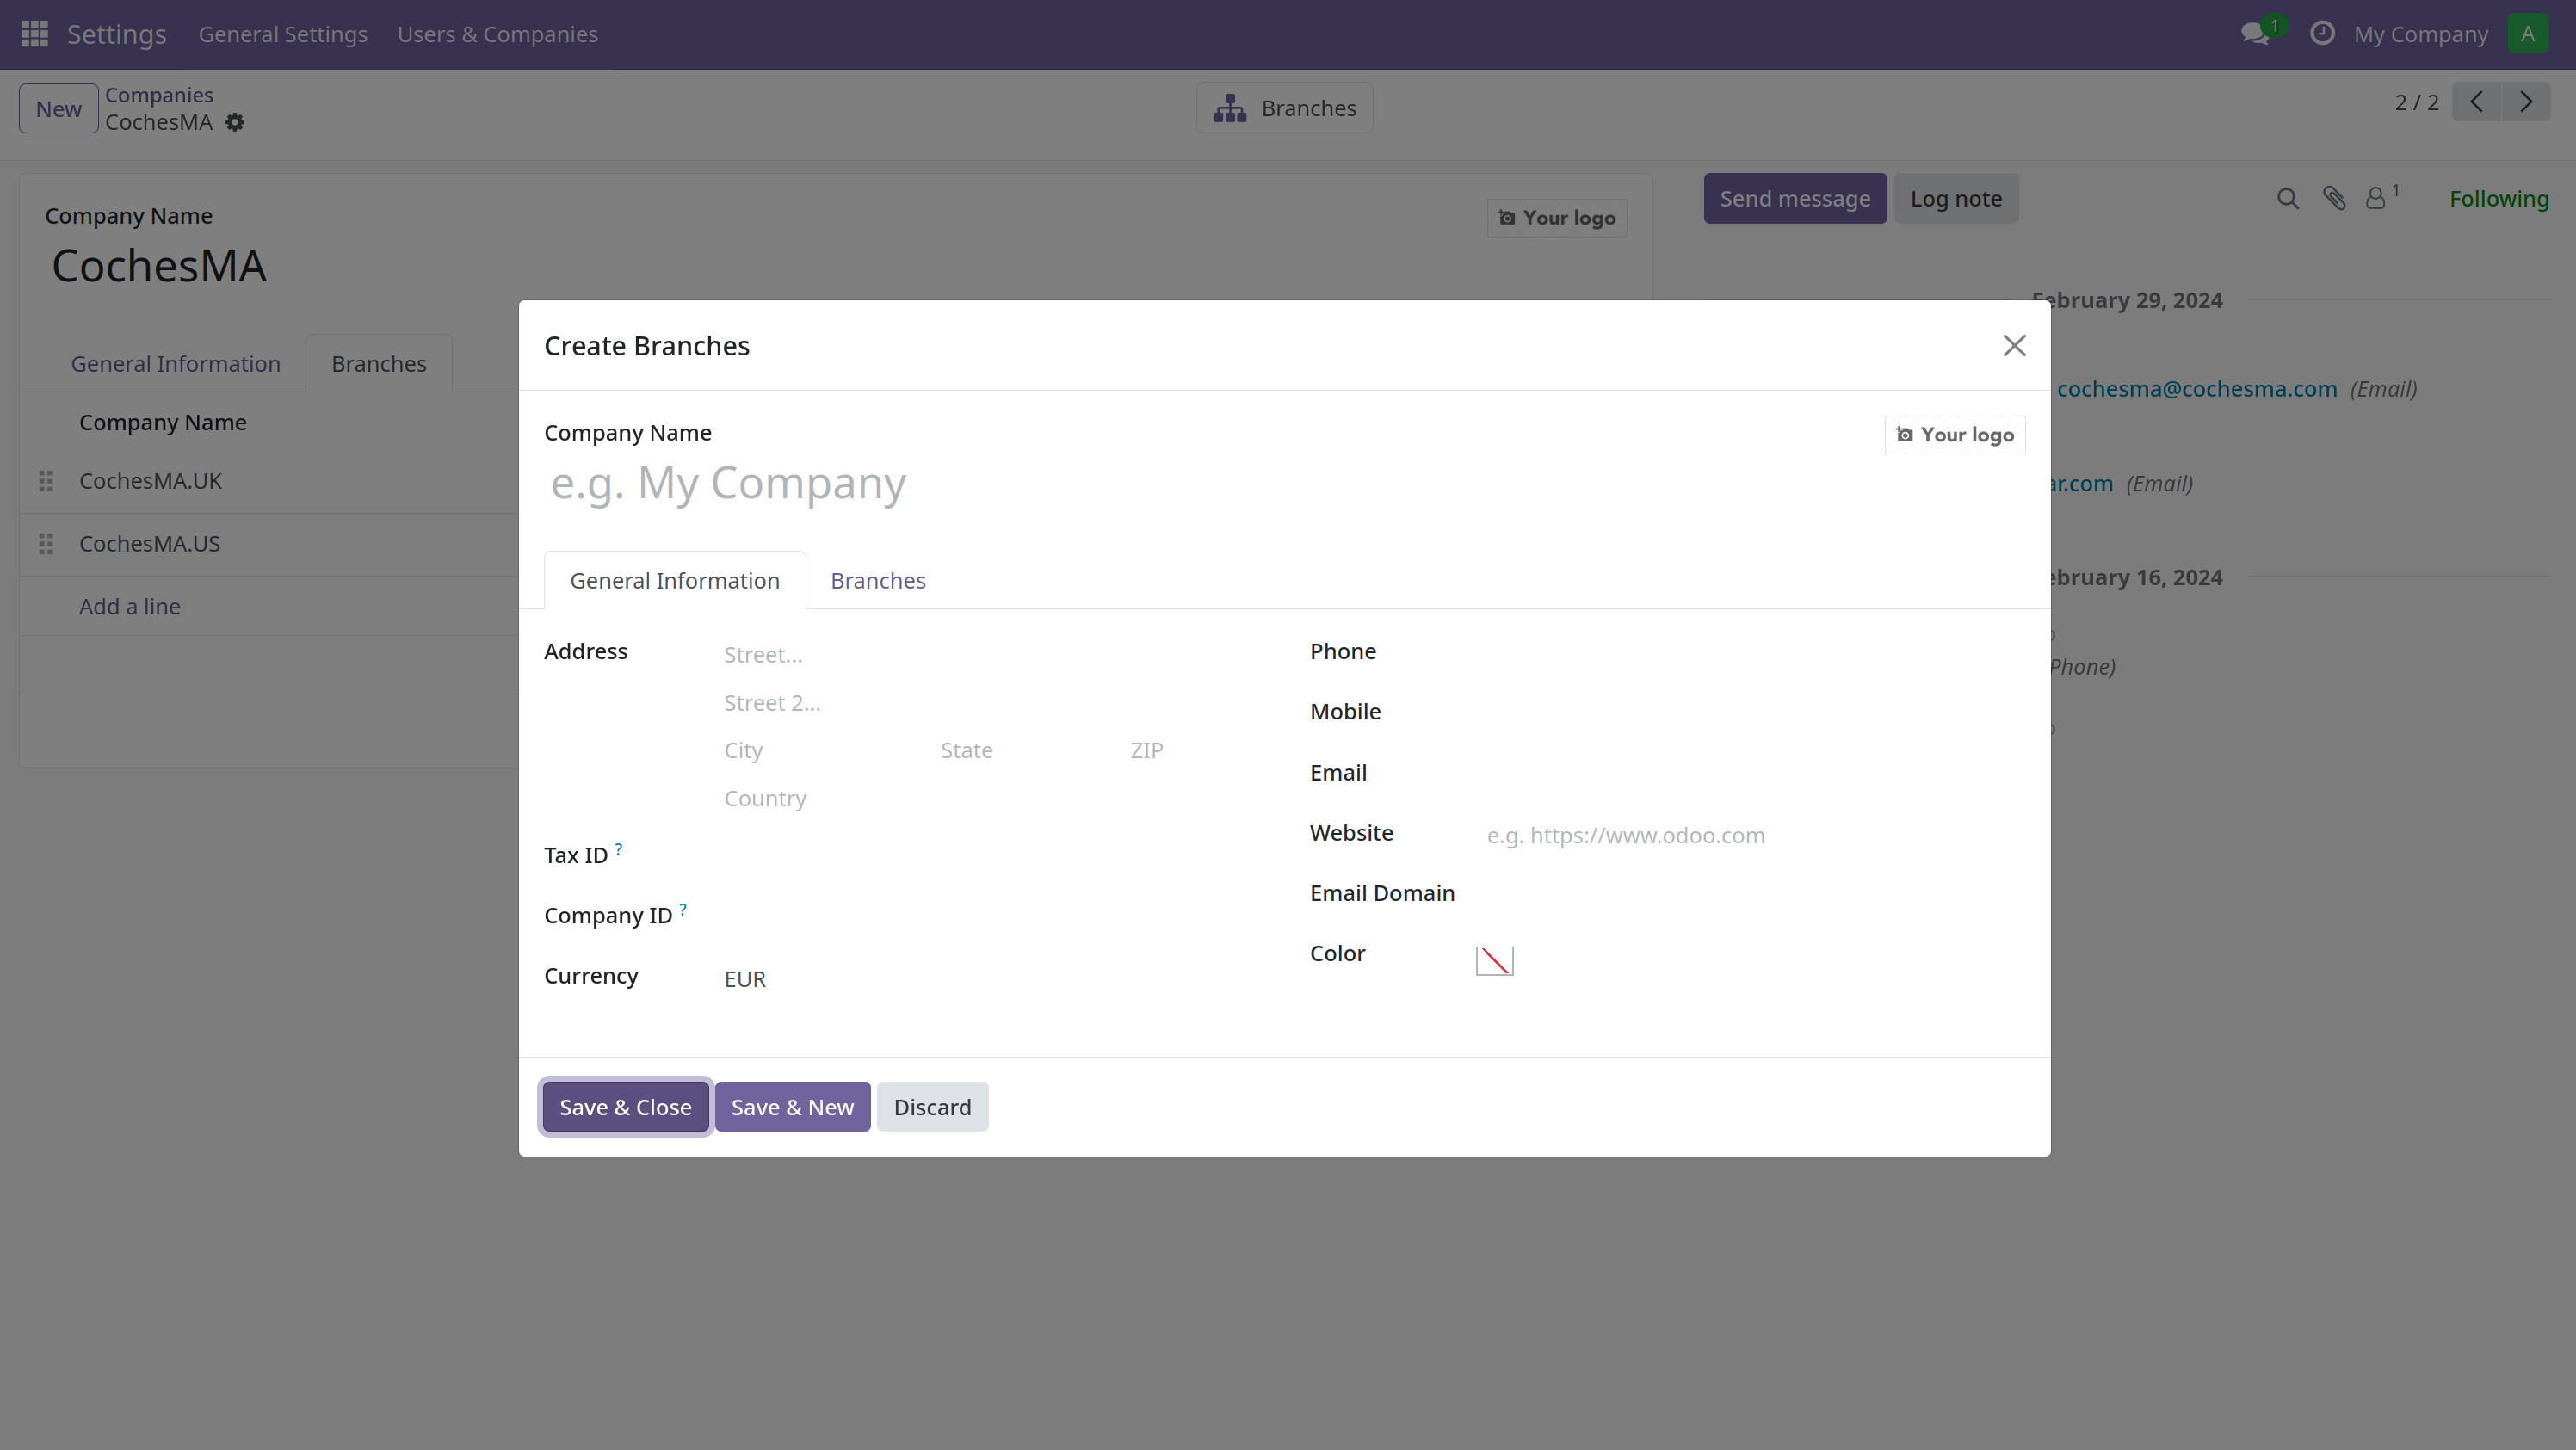
\includegraphics[width=6cm]{crearRama.png}
    \caption{Página de creación de compañías rama.}
    \label{fig:faqs}
\end{figure}
\paragraph{}
Una vez, introducido la información pulsa en Save and Close y se creará la empresa rama, podrás observar que ha aparecido una nueva rama en la página de administración de compañías rama.
\begin{figure}[h]
    \centering
    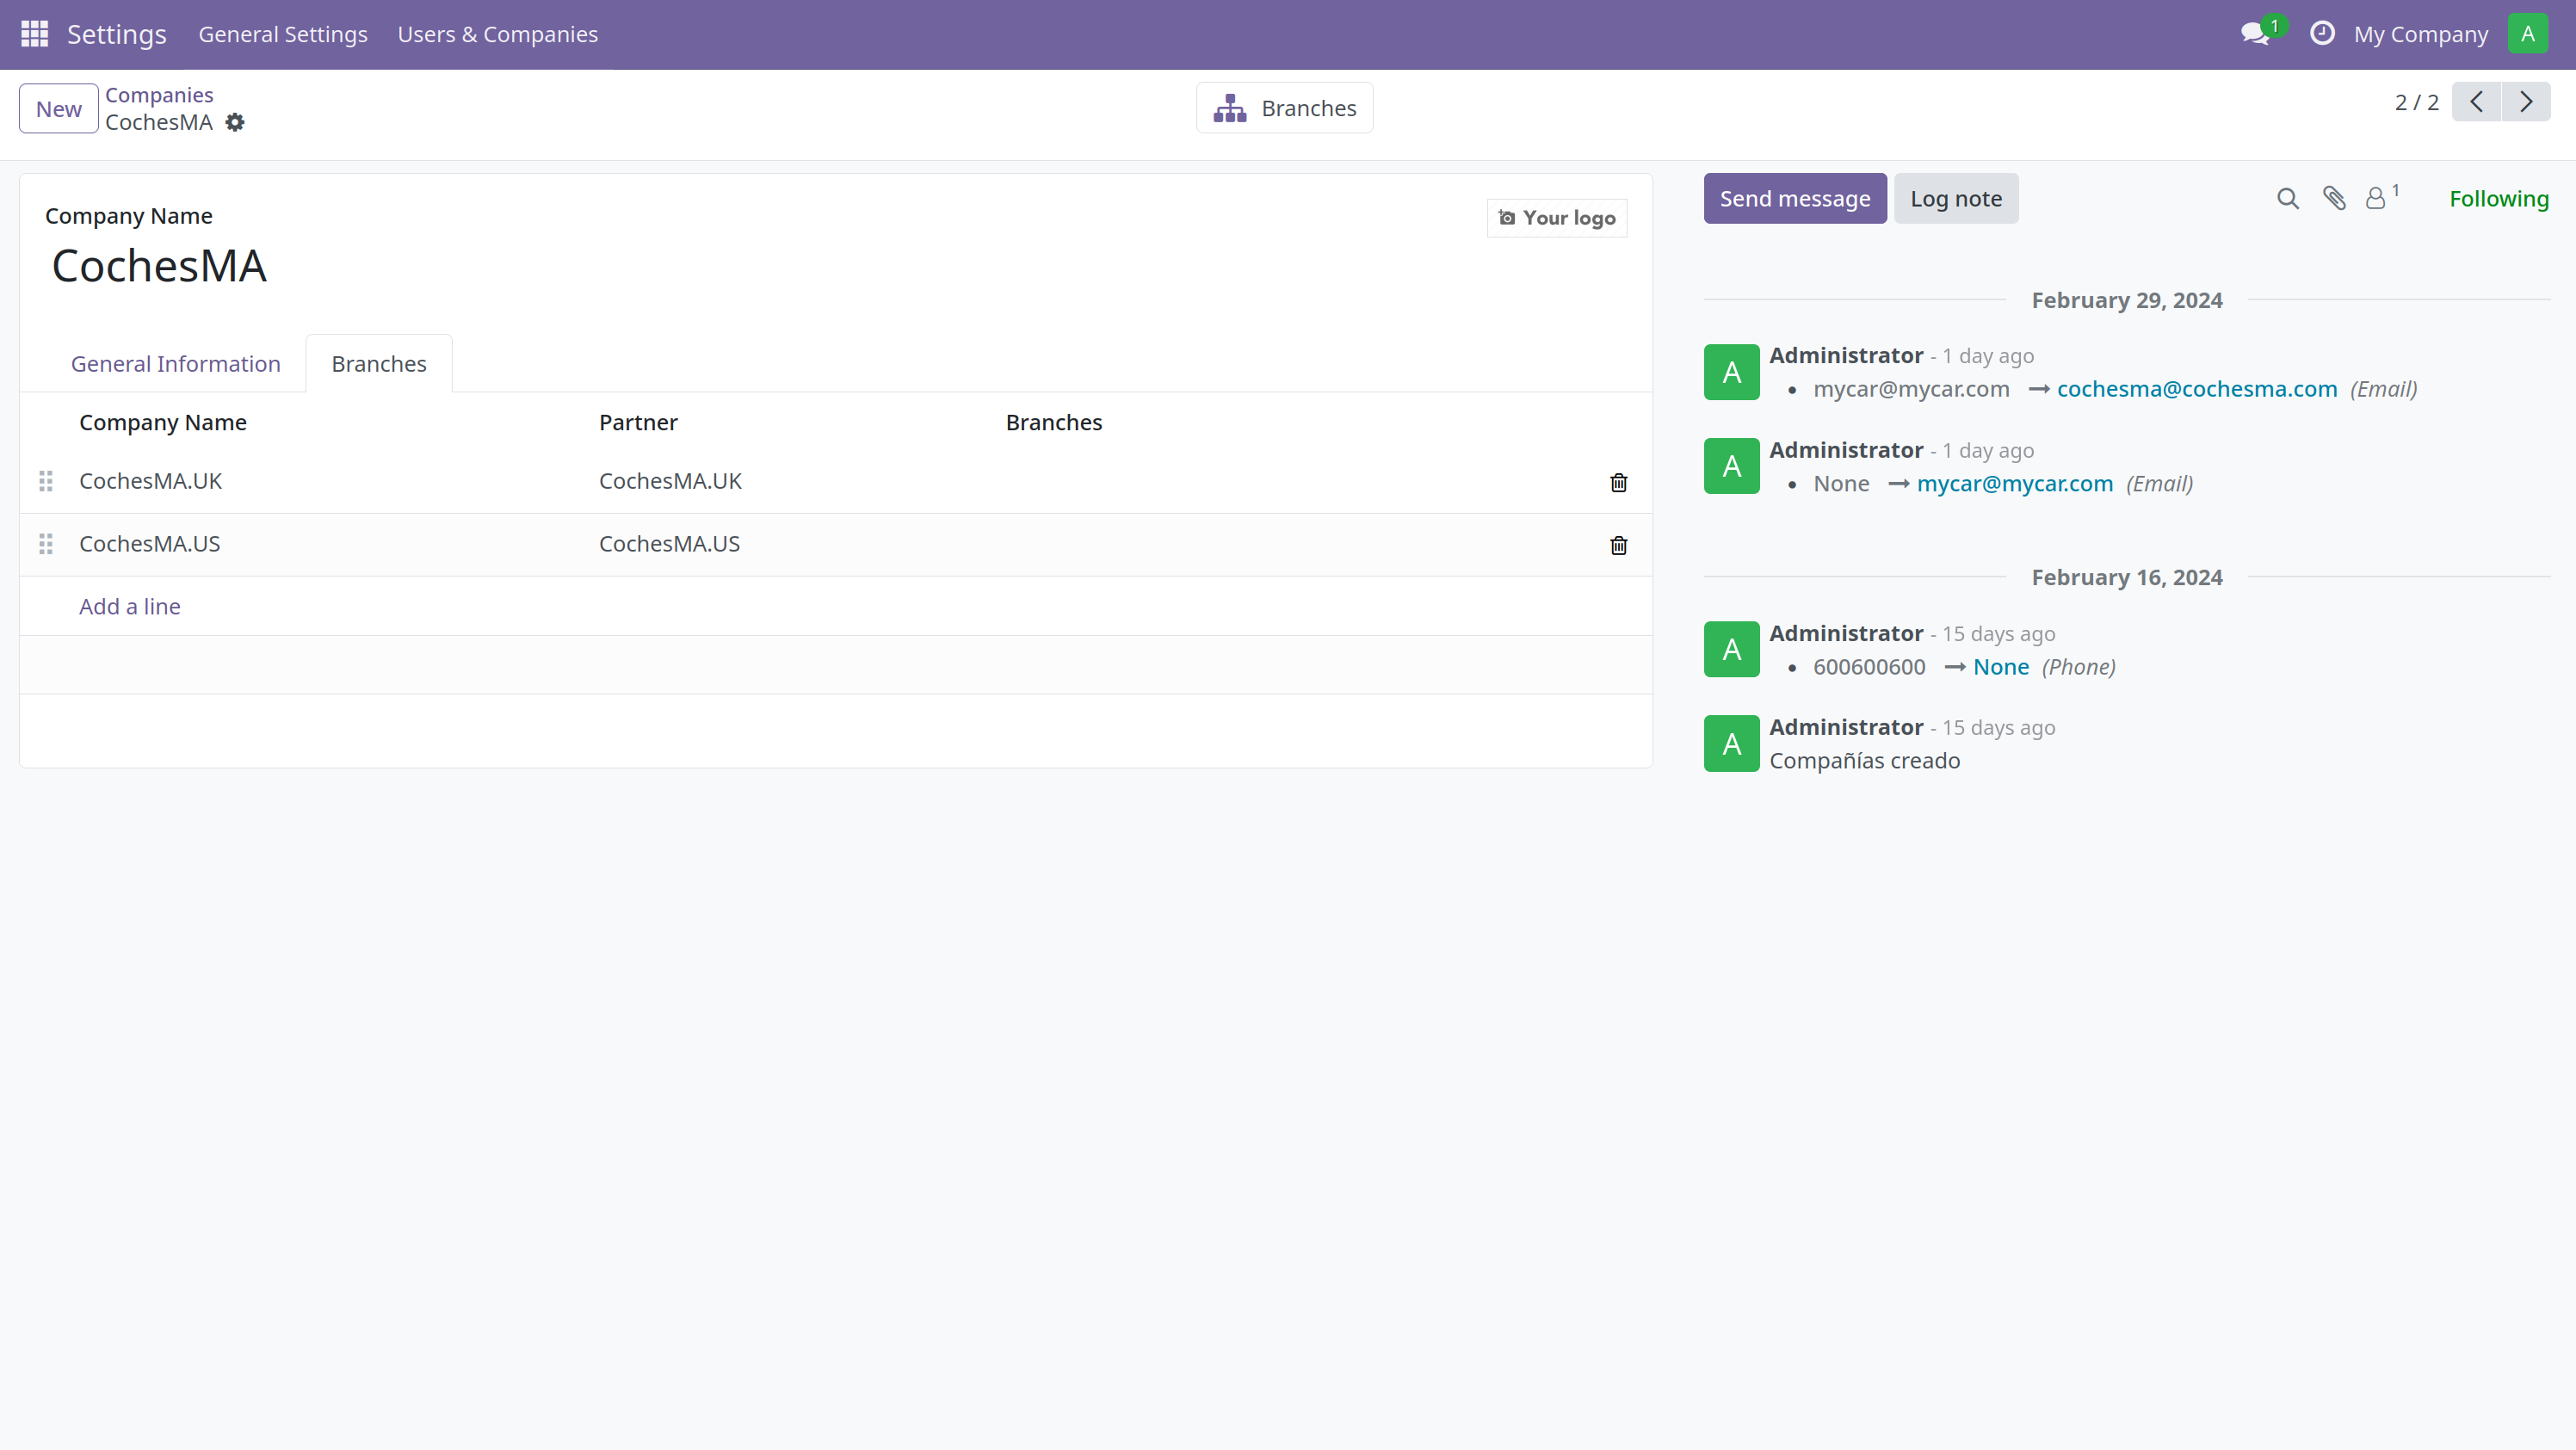
\includegraphics[width=6cm]{ramasCreadas.png}
    \caption{Página de administración de compañías rama con las compañías creadas.}
    \label{fig:faqs}
\end{figure}
\paragraph{}
A continuación, se va a explicar como se pueden crear usuarios para las compañías, tanto la matríz como las ramas. Como aparece en la figura 10, pulsa en el link Administrar usuarios y pulsa en New de la esquina superior izquierda. 
\begin{figure}[h]
    \centering
    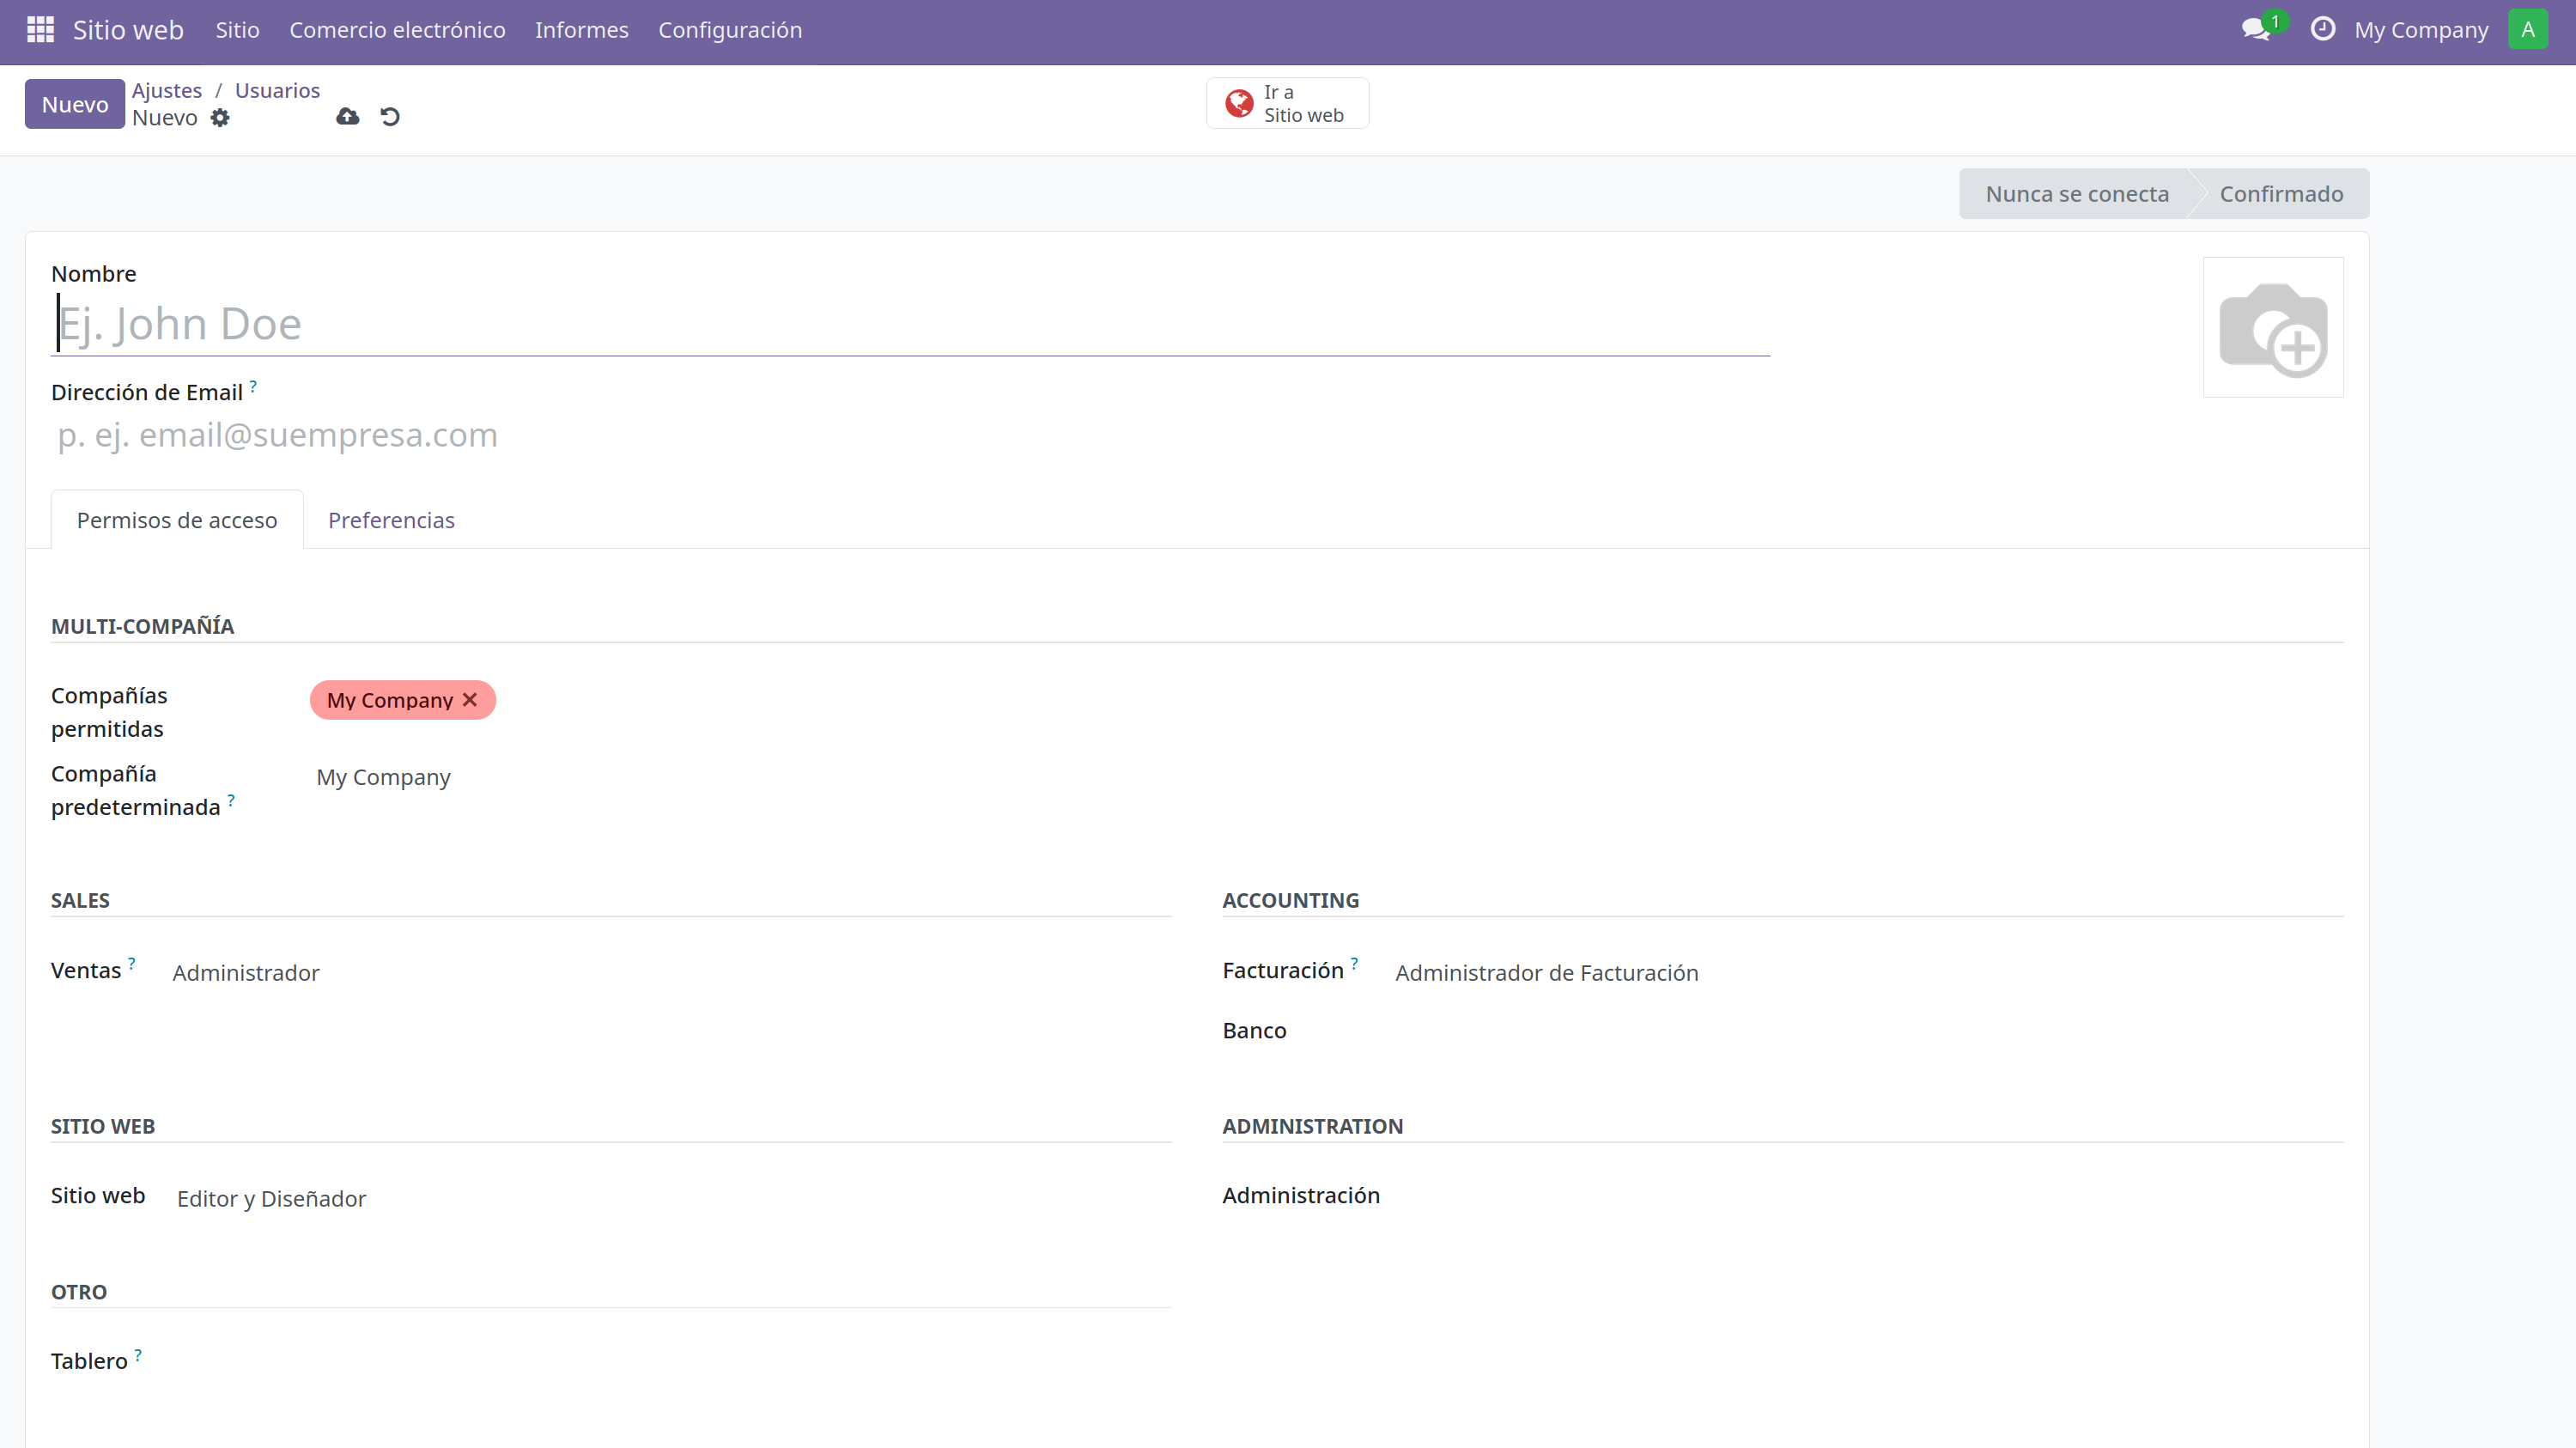
\includegraphics[width=6cm]{adminUsuarios.png}
    \caption{Página de usuarios de la compañía.}
    \label{fig:faqs}
\end{figure}
\paragraph{}




\end{document} 
